%----------------------------------------------------------------------------------------------
%-----------------------     7 Anwendungsbeispiele aus der Vorlesung    -----------------------
%----------------------------------------------------------------------------------------------
\section{Anwendungsbeispiele aus der Vorlesung}
% Hier sind bewusst nur die Folien aus den Vorlesungen eingefügt, damit auf der ausgedrucken Form der 
% Zusammenfassung individuelle Notizen gemacht werden können
		 

%----------------------------------------------------------------------------------------------
%------------------------------------     7.1 Matrixoptik    ----------------------------------
%----------------------------------------------------------------------------------------------
\subsection{Matrixoptik}

\begin{center}
	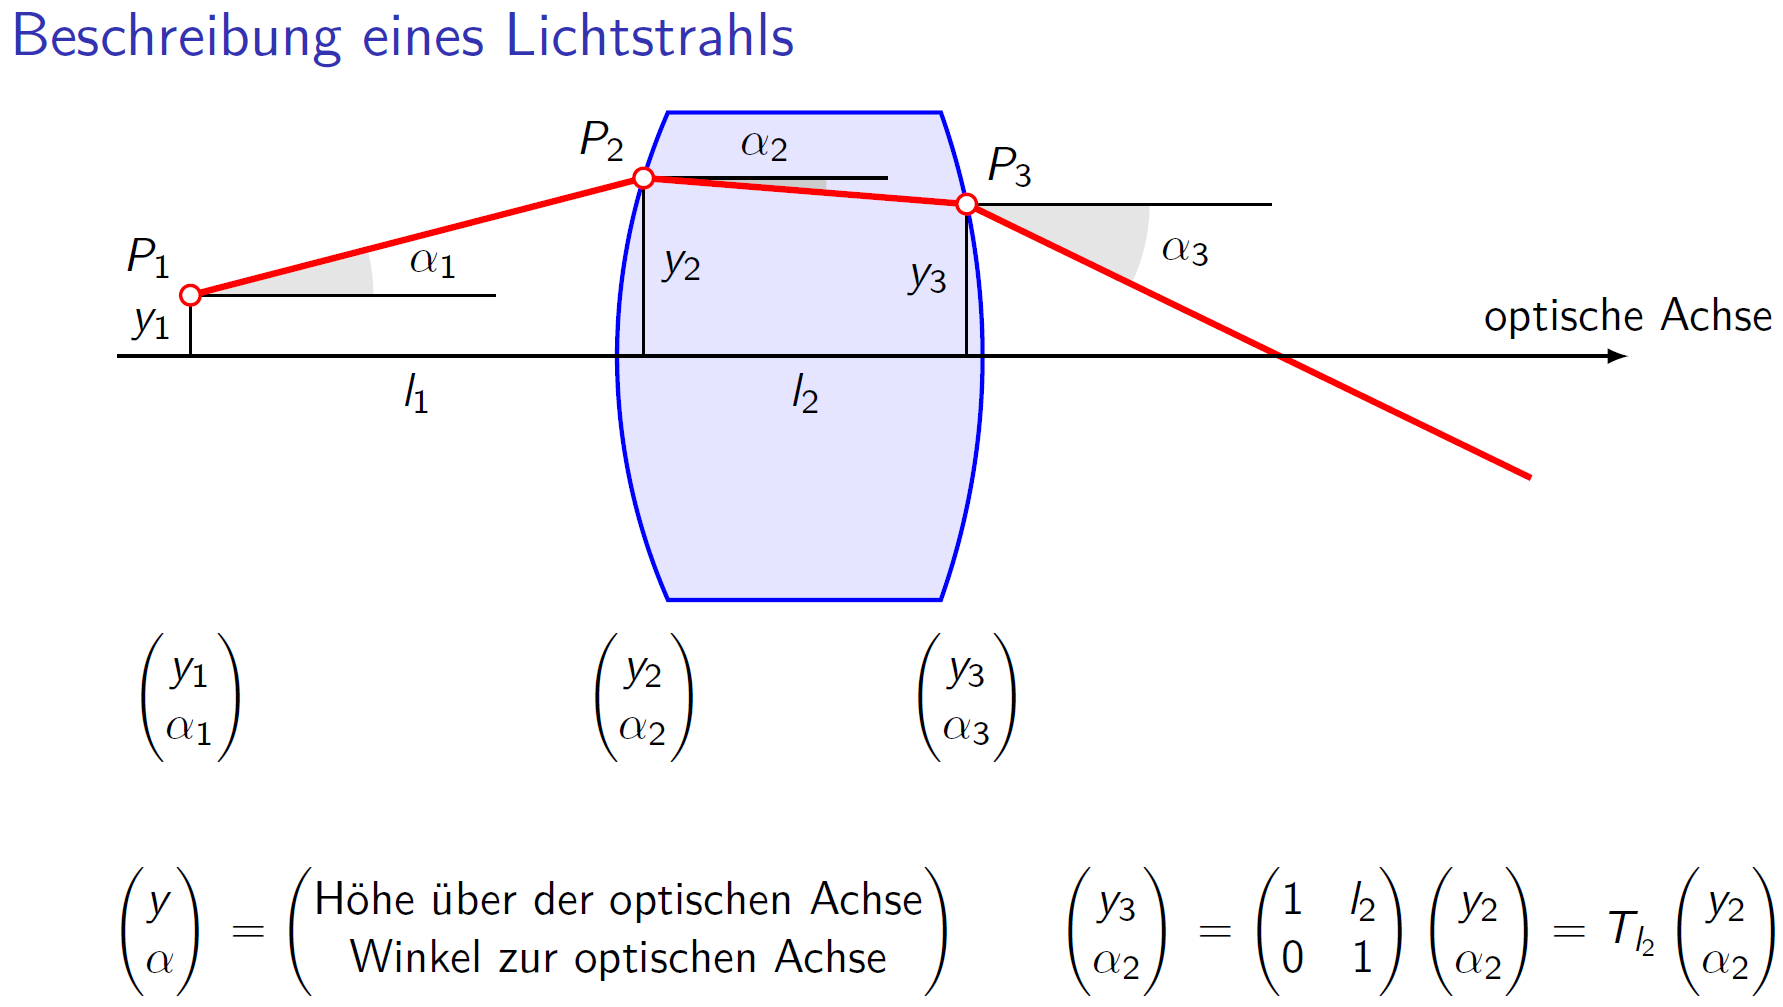
\includegraphics[width=0.8\columnwidth]{images/matrixoptik1.PNG}		
	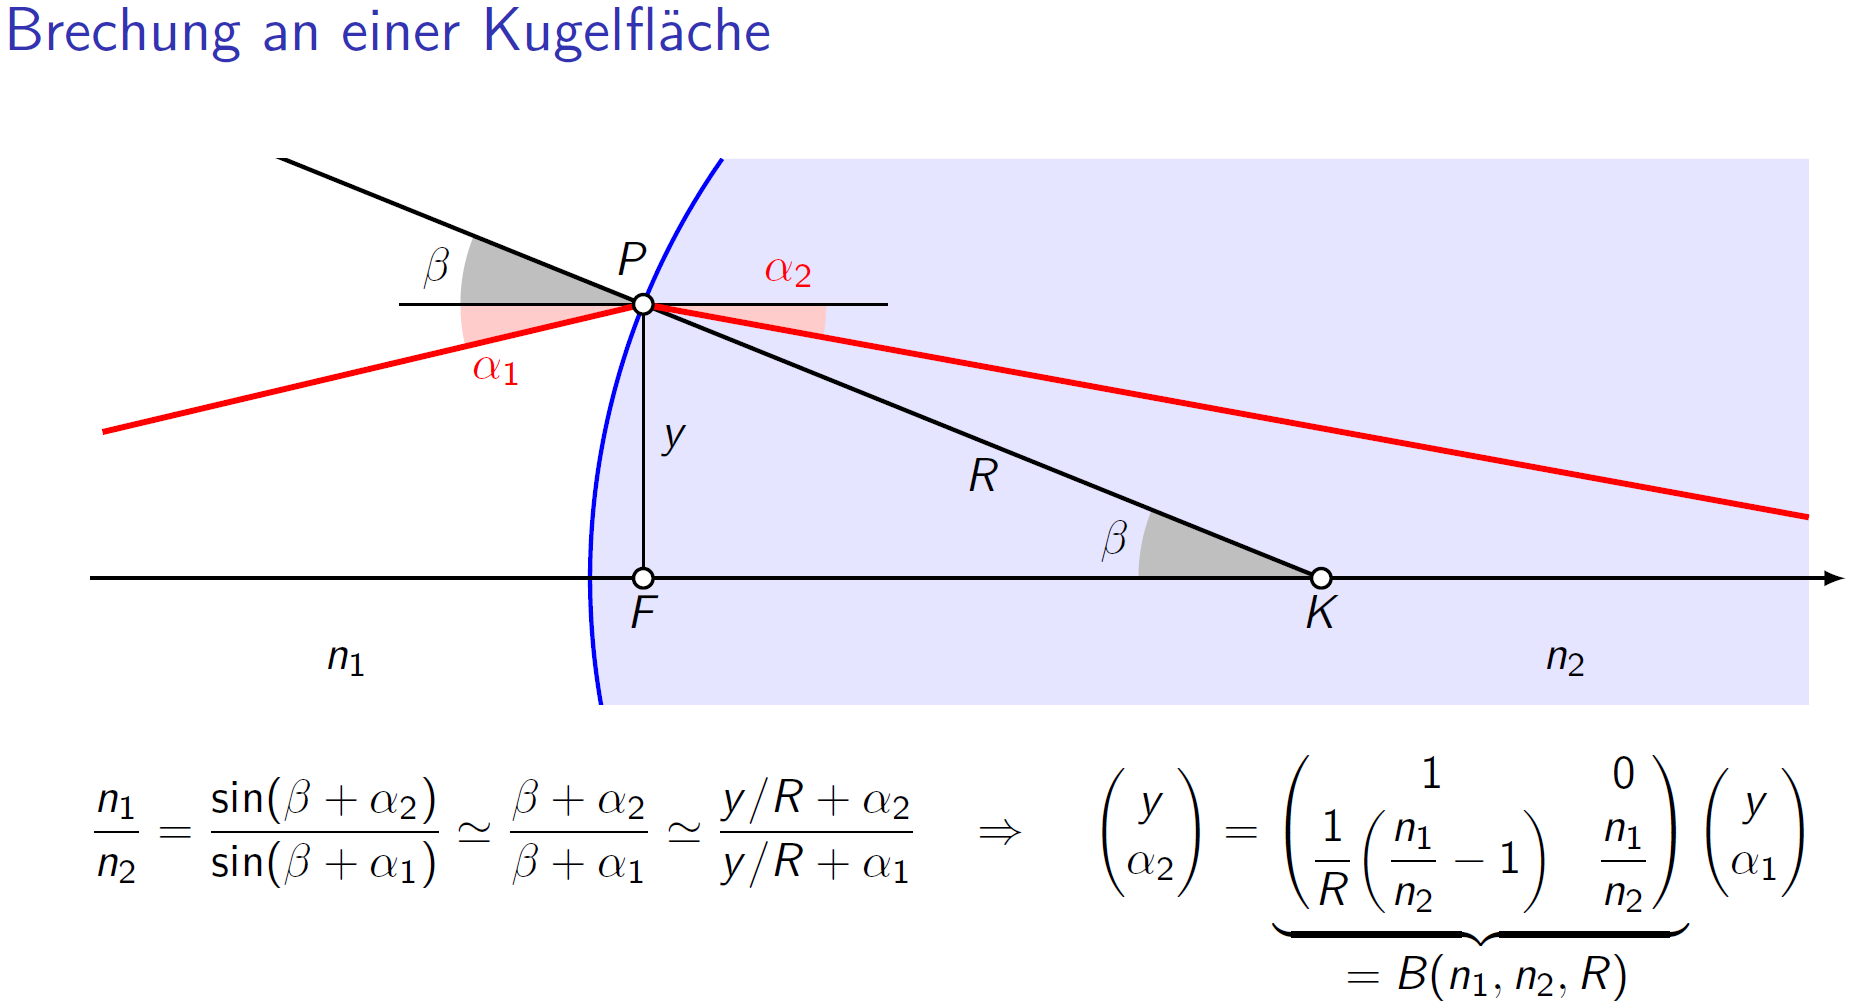
\includegraphics[width=0.8\columnwidth]{images/matrixoptik2.PNG}
	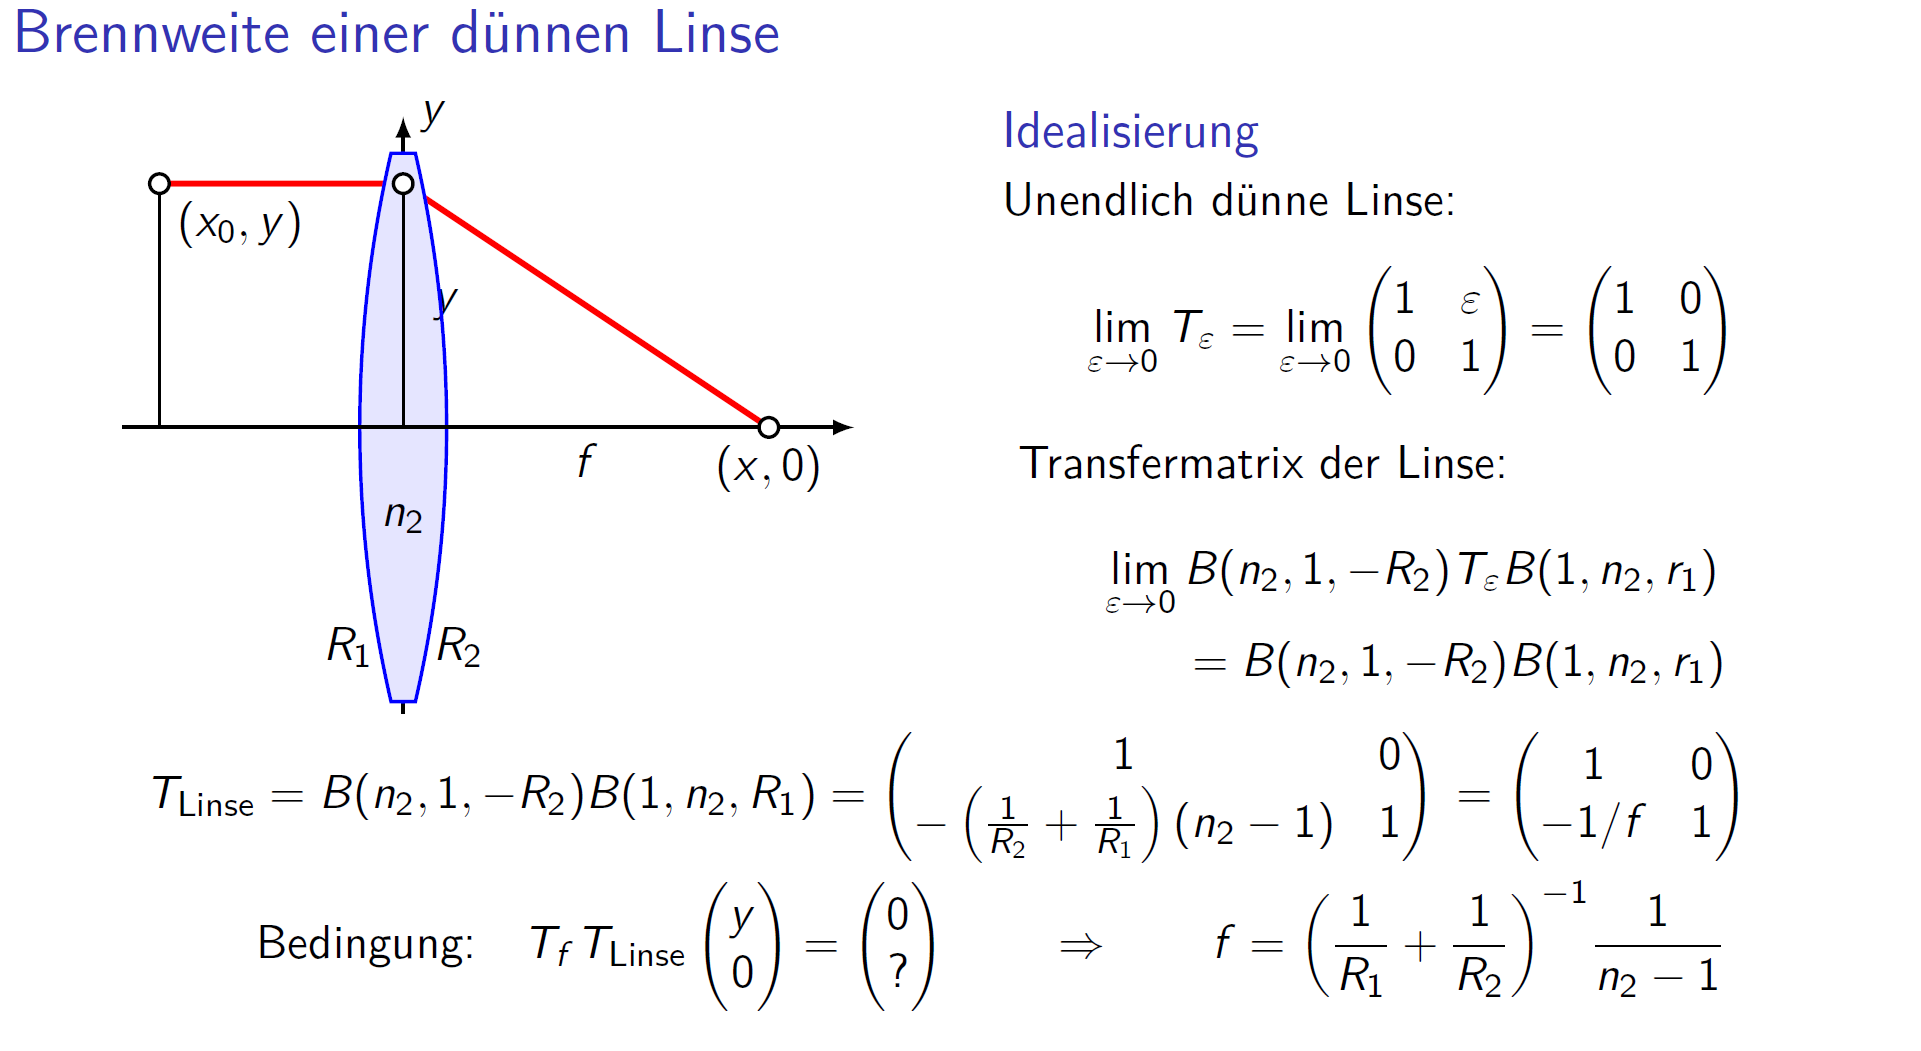
\includegraphics[width=0.8\columnwidth]{images/matrixoptik3.PNG}
	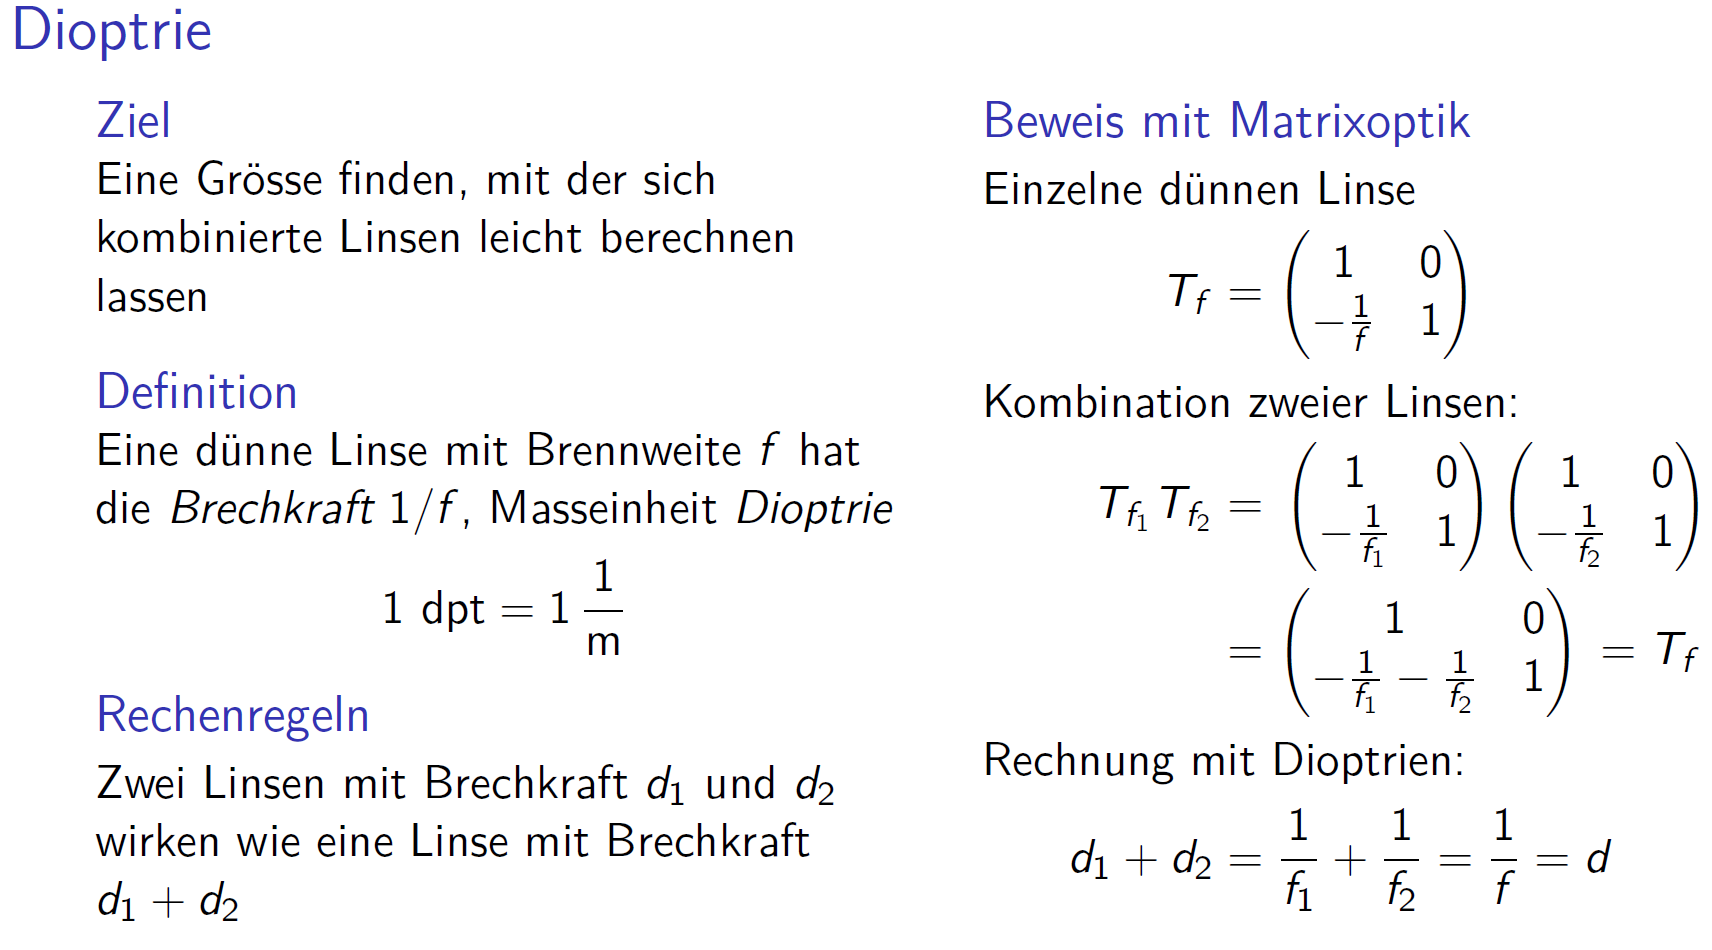
\includegraphics[width=0.8\columnwidth]{images/matrixoptik4.PNG}
	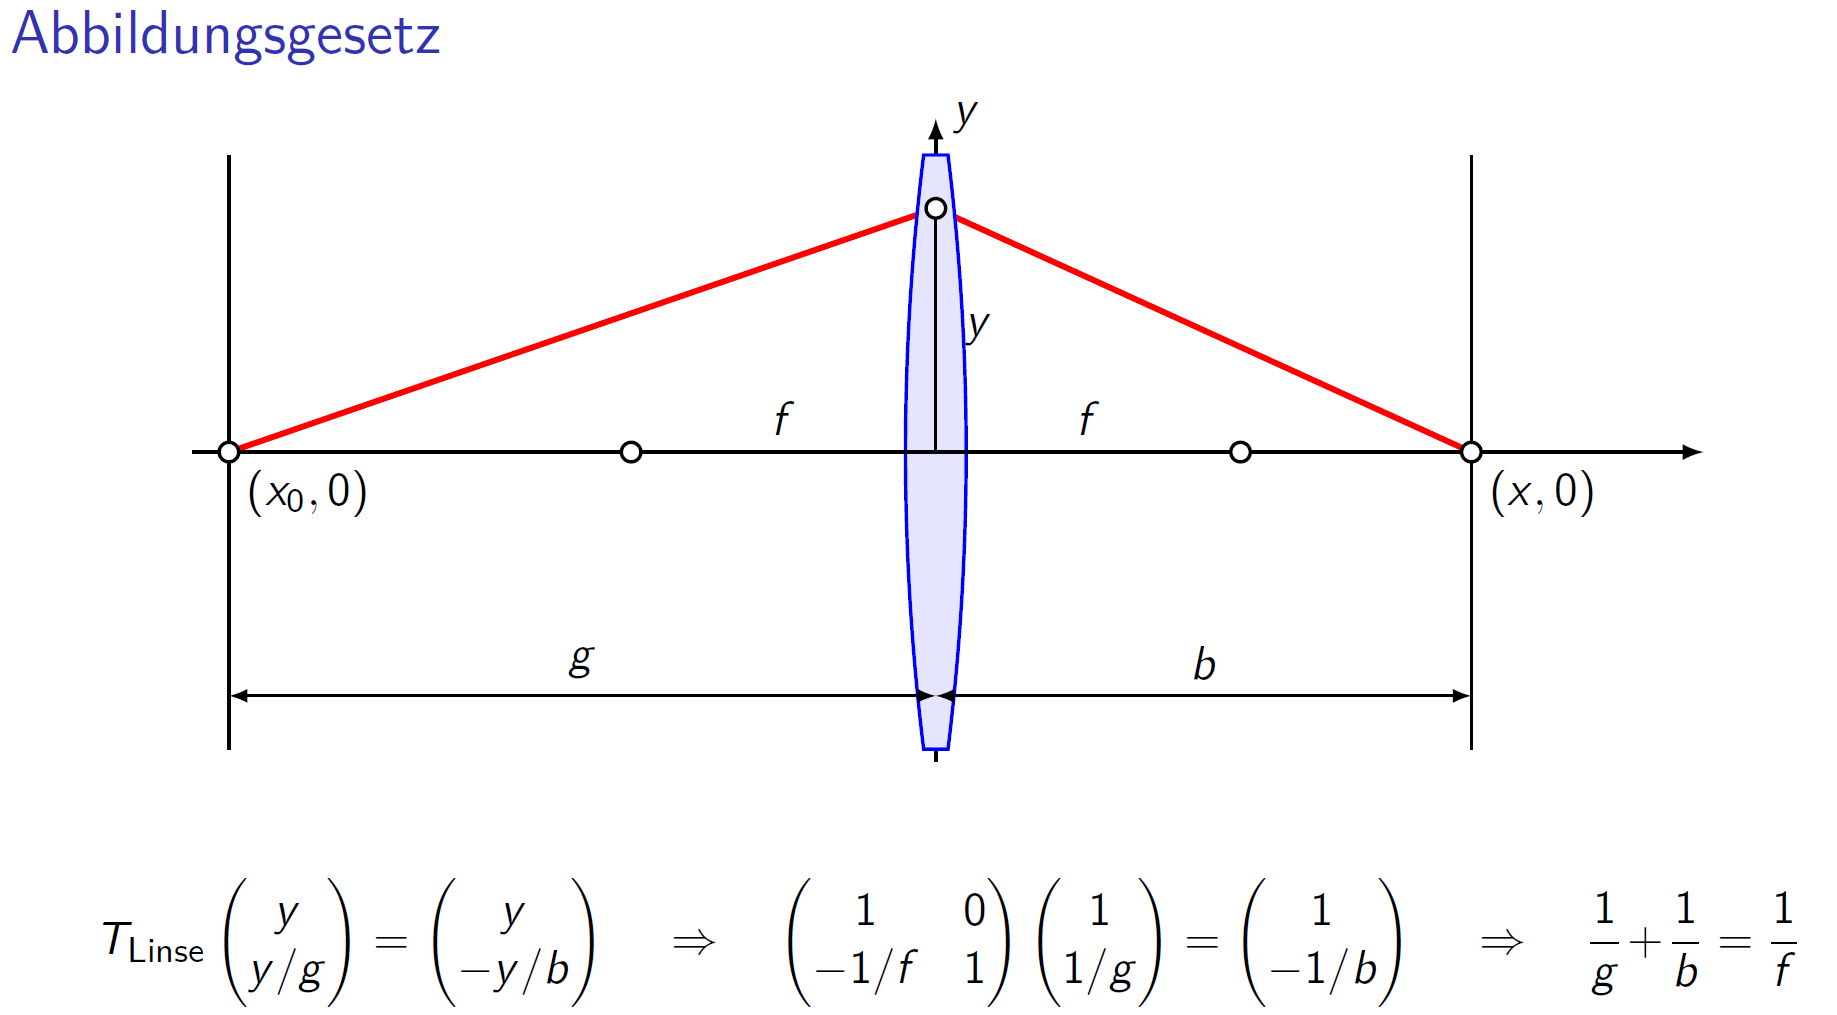
\includegraphics[width=0.8\columnwidth]{images/matrixoptik5.PNG}
	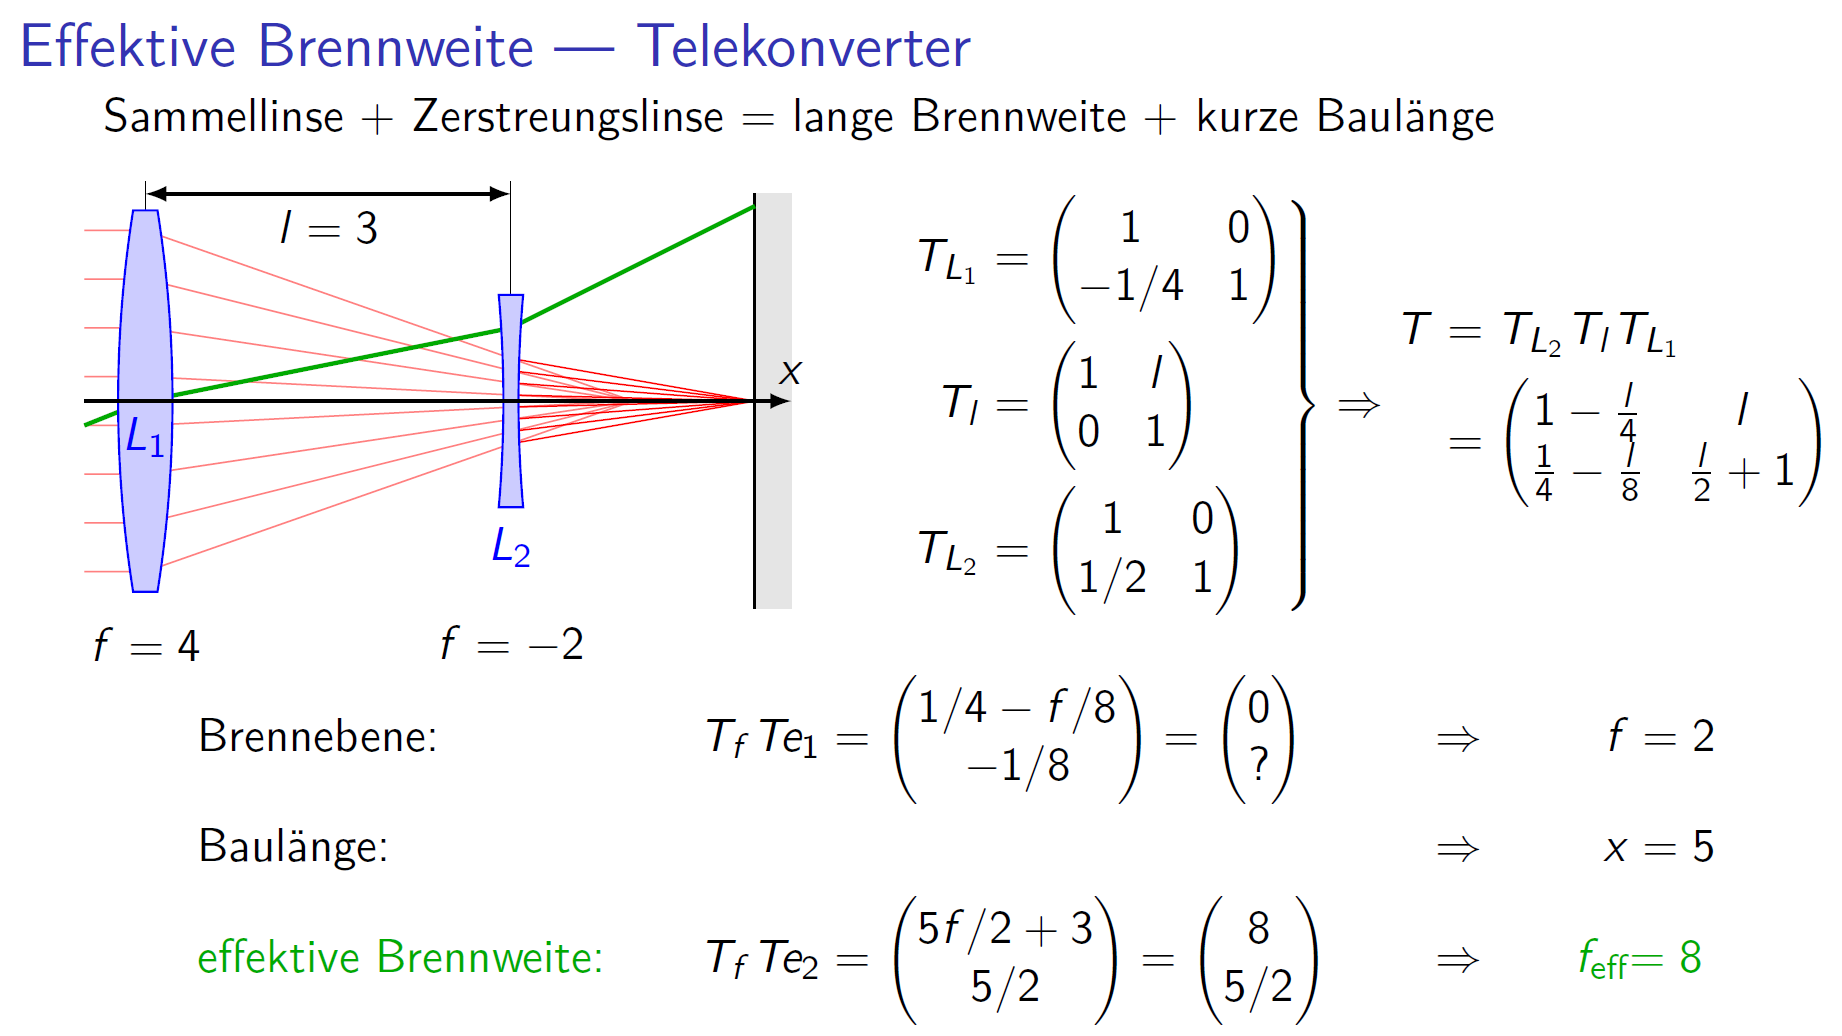
\includegraphics[width=0.8\columnwidth]{images/matrixoptik6.PNG}
\end{center}


%----------------------------------------------------------------------------------------------
%-----------------------------------     7.2 Kettenbrüche    ----------------------------------
%----------------------------------------------------------------------------------------------
\subsection{Kettenbrüche}

\begin{center}
	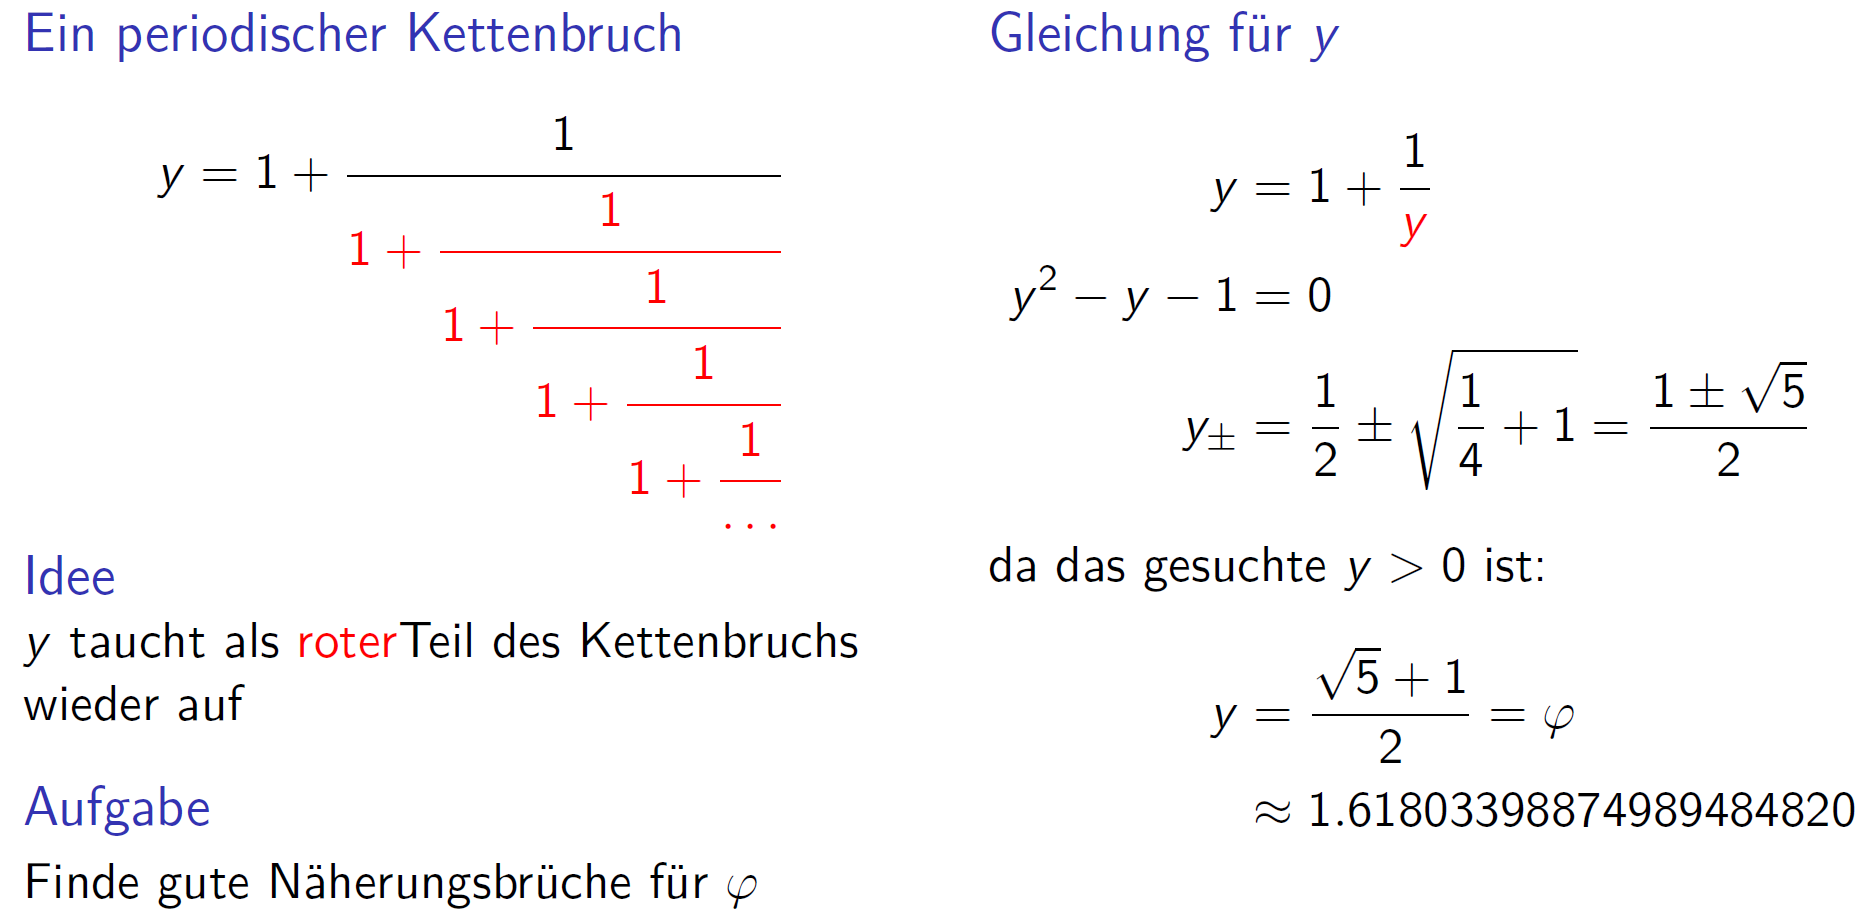
\includegraphics[width=0.8\columnwidth]{images/kettenbruch1.PNG}
	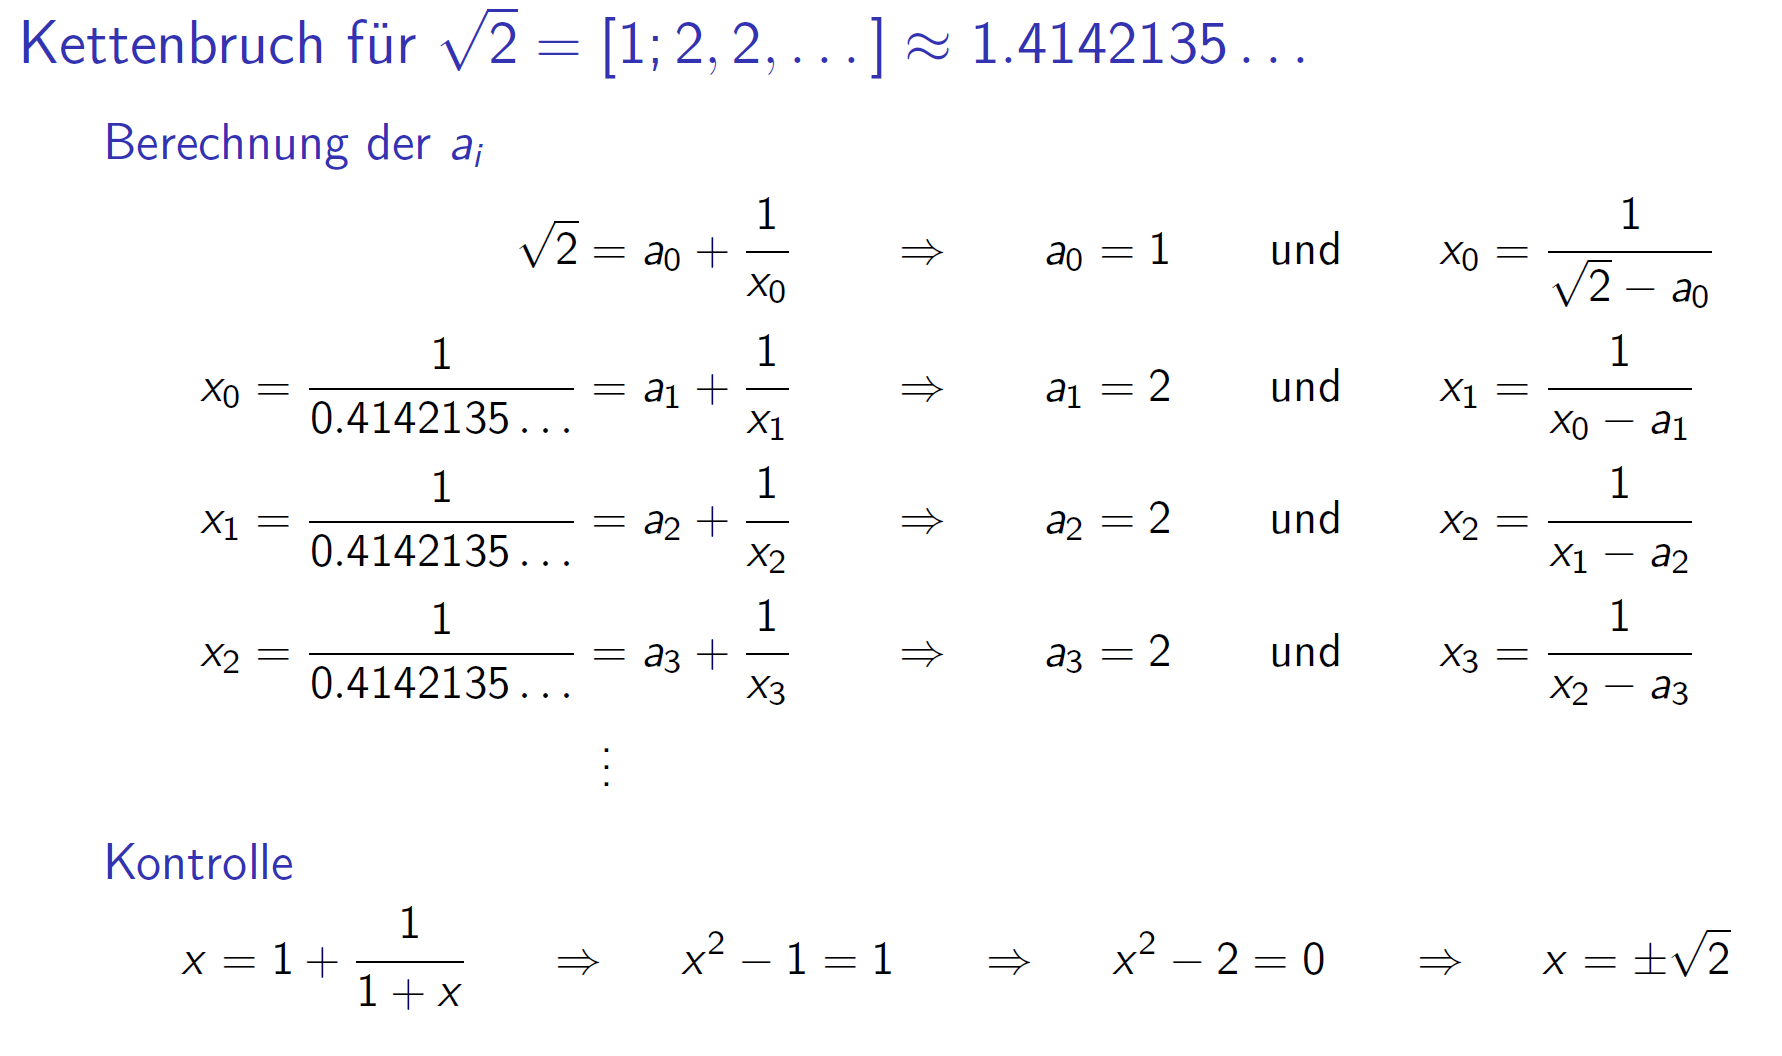
\includegraphics[width=0.8\columnwidth]{images/kettenbruch2.PNG}
	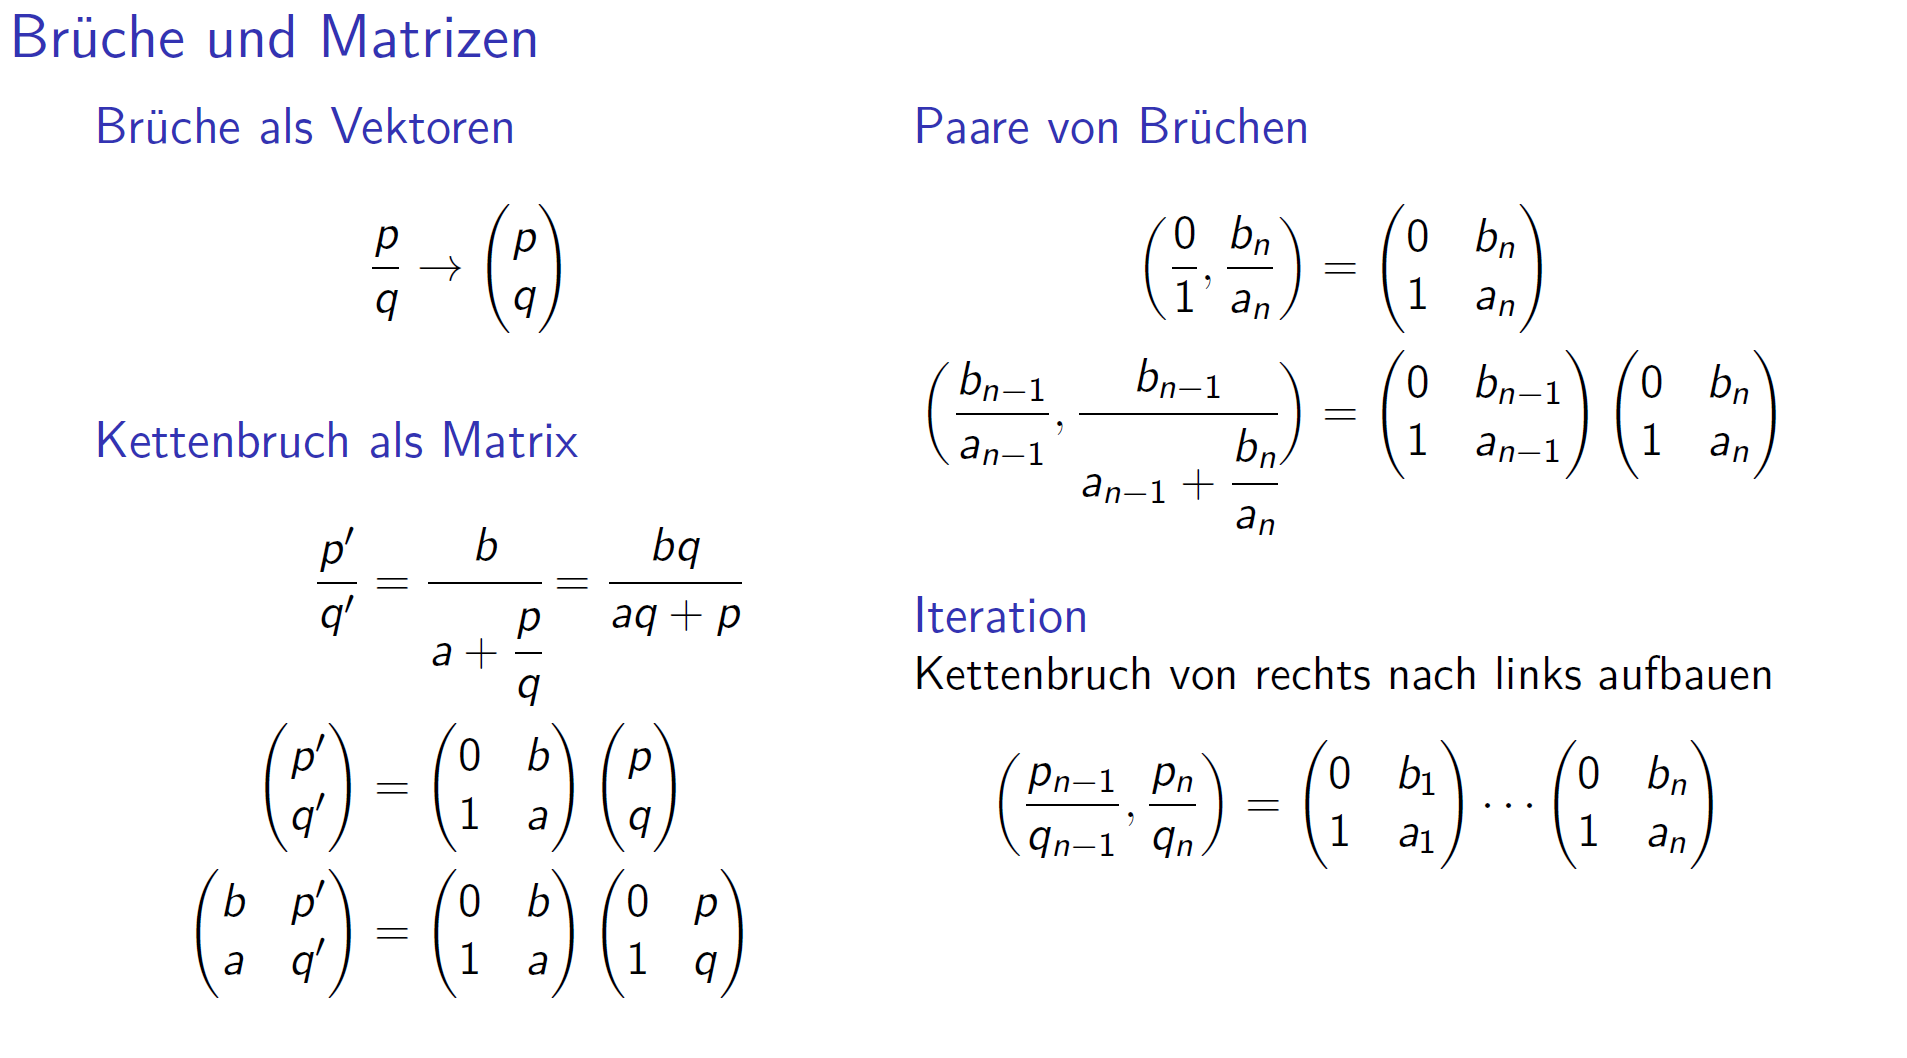
\includegraphics[width=0.8\columnwidth]{images/kettenbruch3.PNG}
	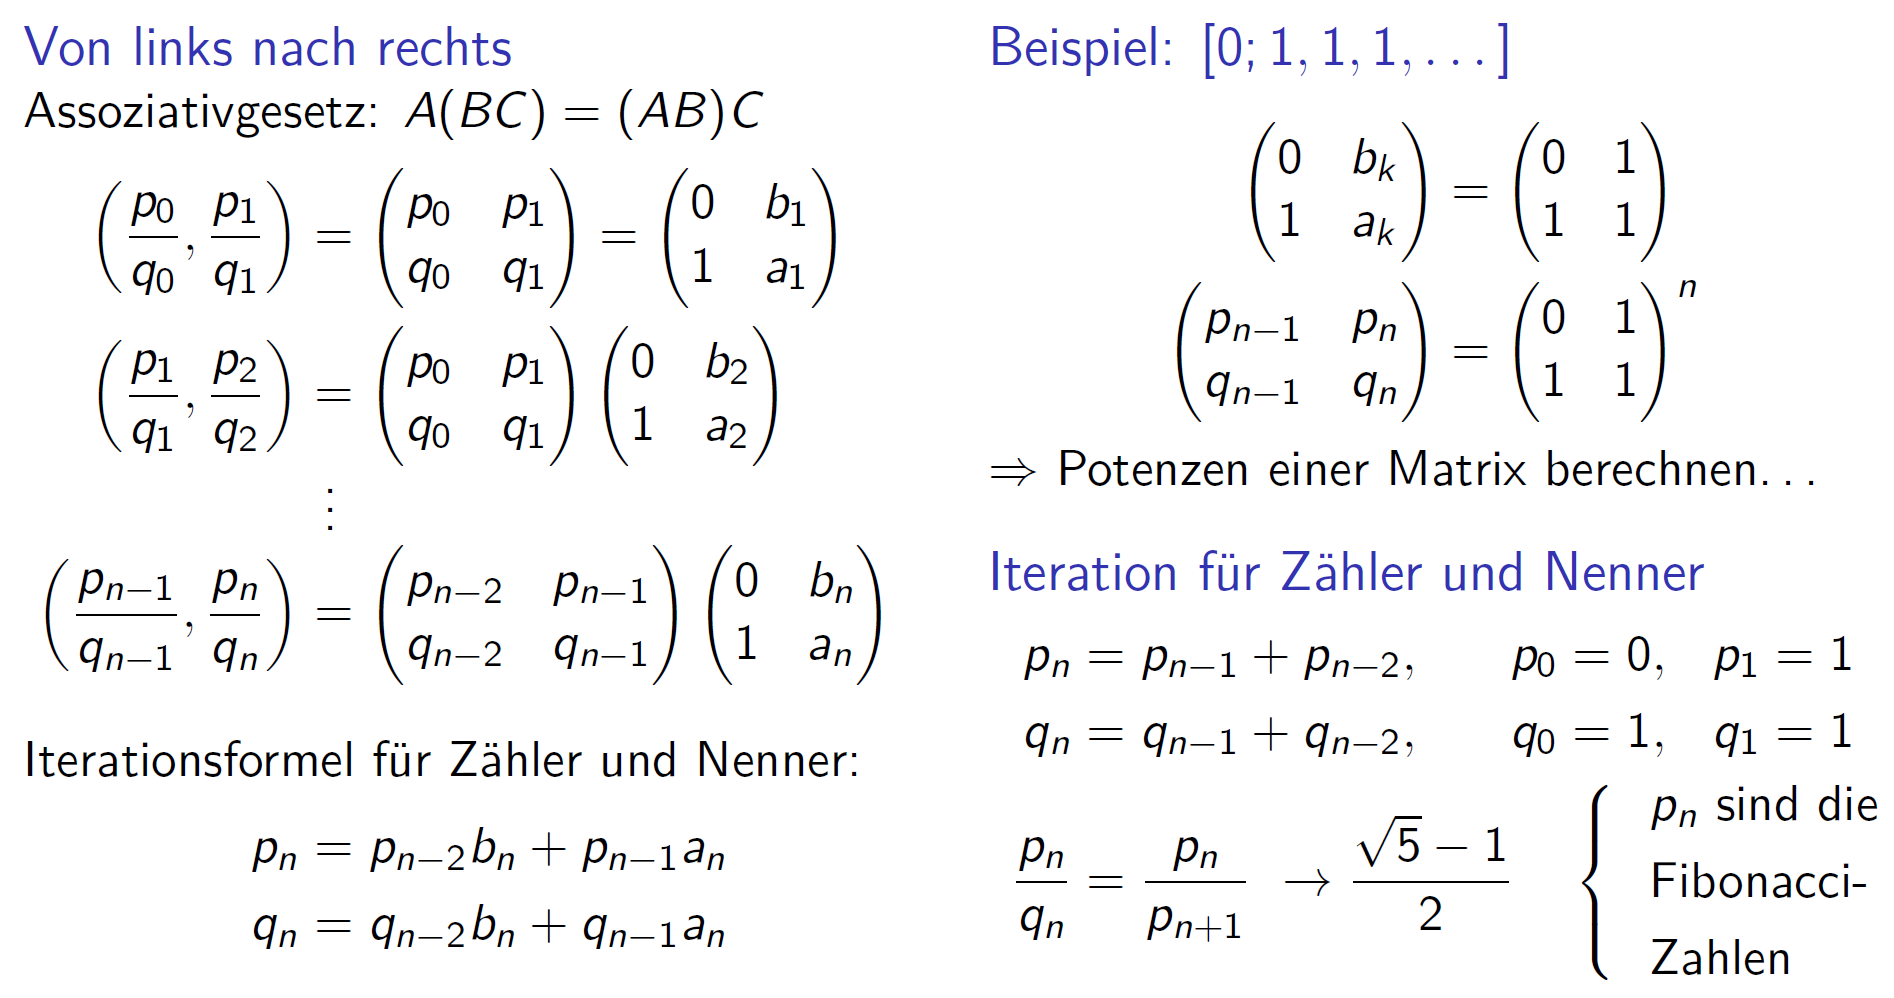
\includegraphics[width=0.8\columnwidth]{images/kettenbruch4.PNG}
	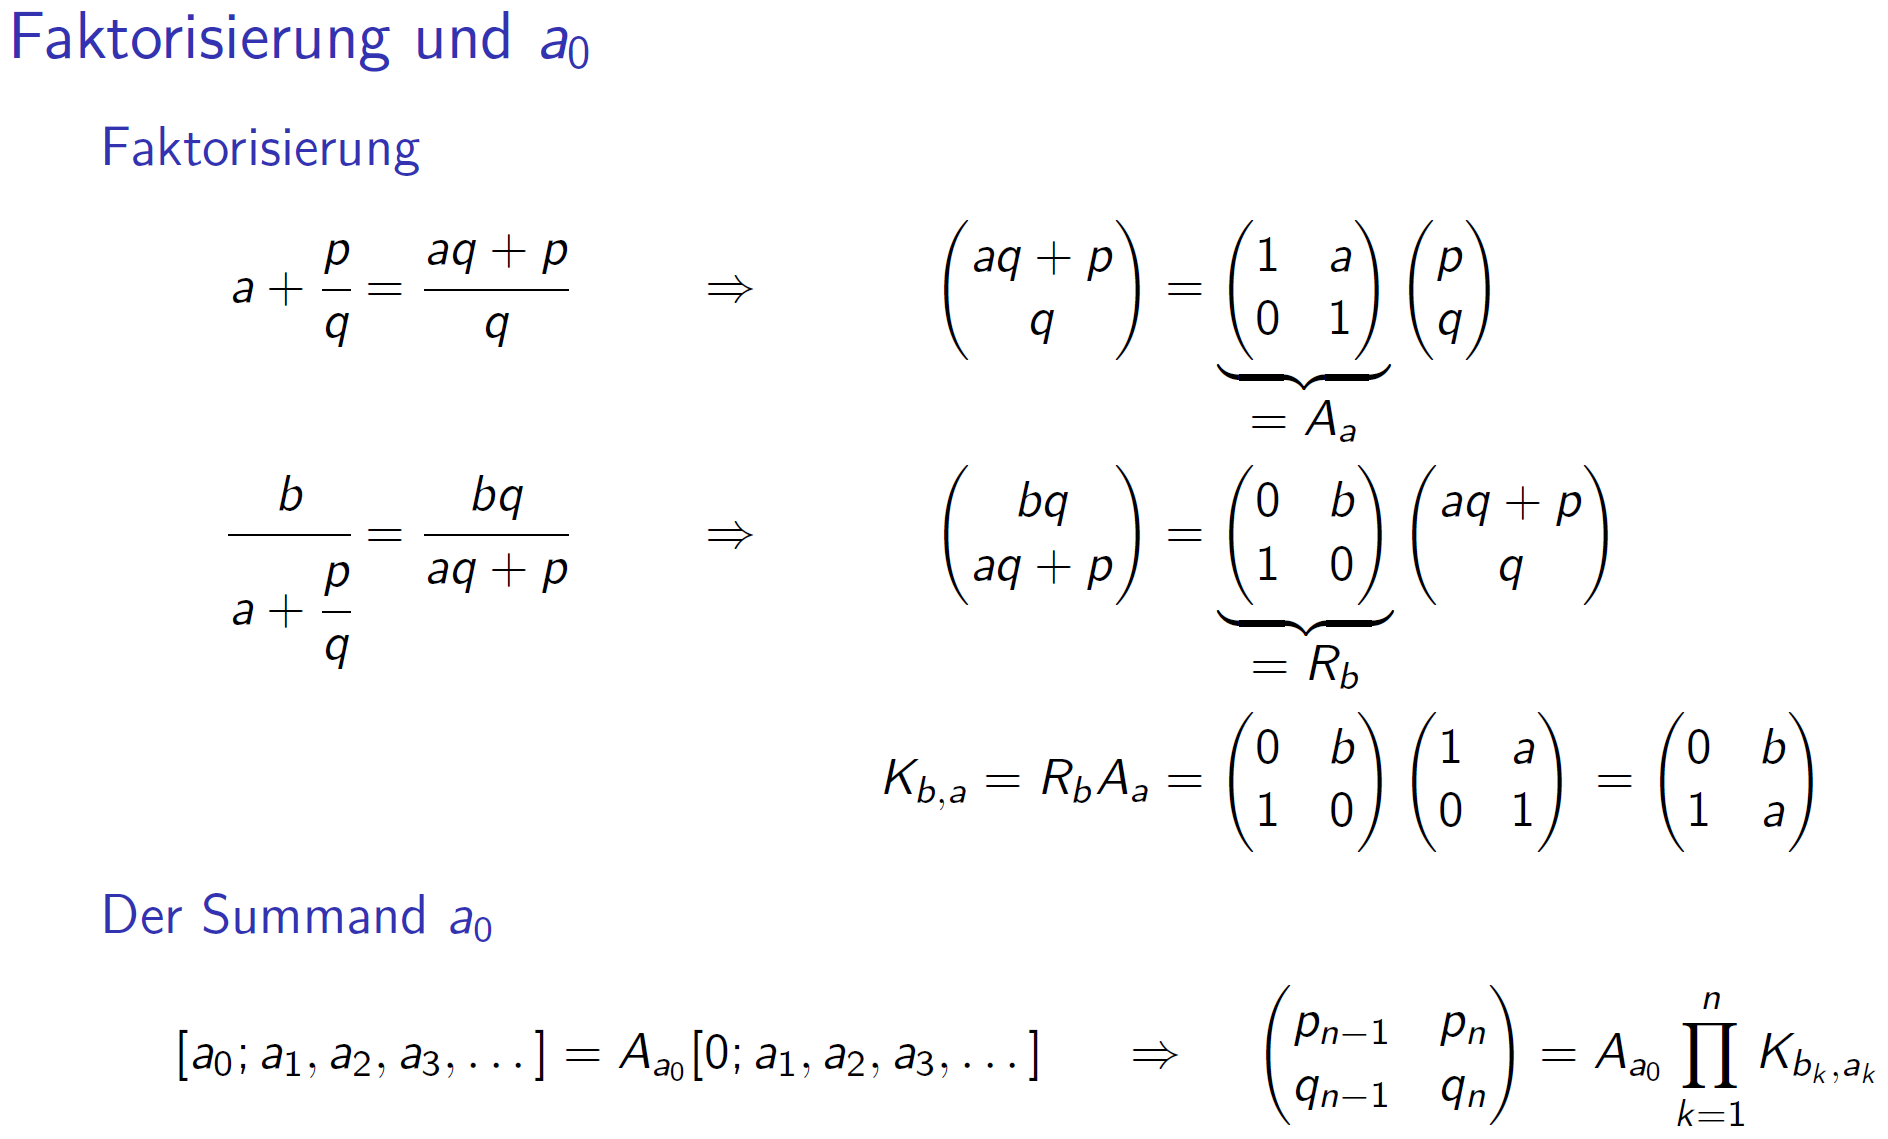
\includegraphics[width=0.8\columnwidth]{images/kettenbruch5.PNG}
\end{center}


%----------------------------------------------------------------------------------------------
%---------------------------------     7.3 Rekursionsformeln    -------------------------------
%----------------------------------------------------------------------------------------------
\subsection{Rekursionsformeln}

\textbf{Anwendung Eigenwerte / Eigenvektoren / Eigenbasis}
\begin{center}
	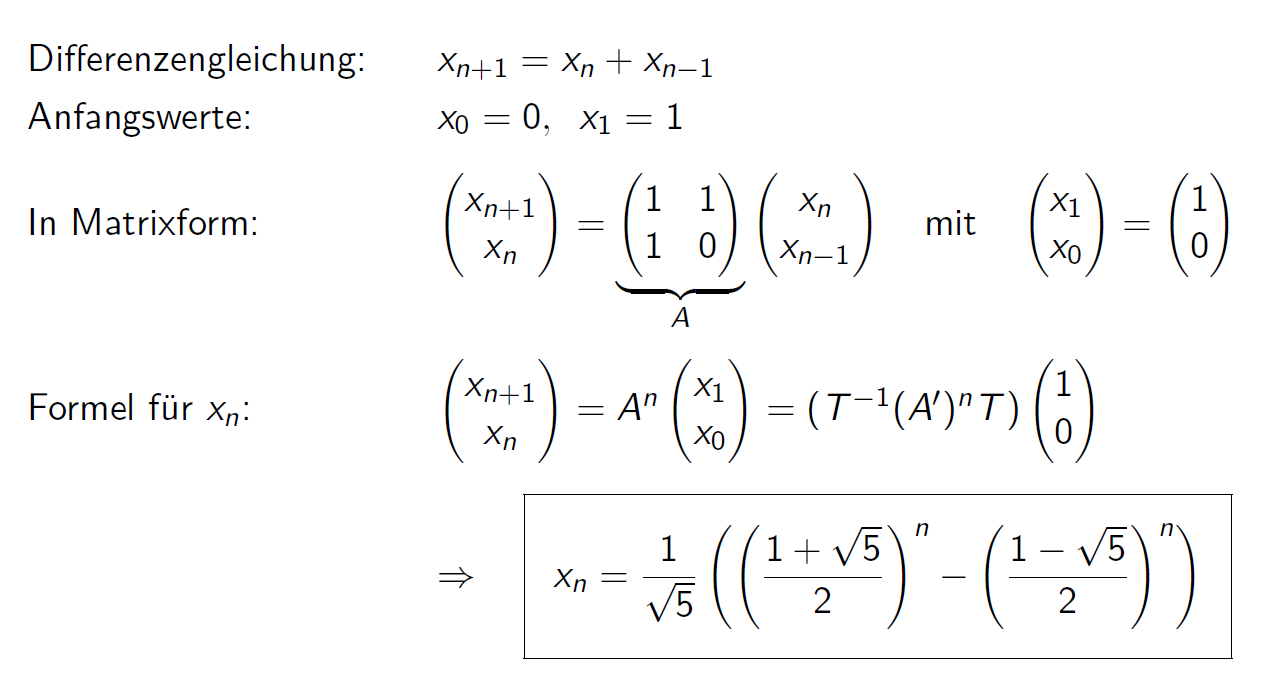
\includegraphics[width=0.75\columnwidth]{images/rekursion1.PNG} 
\end{center}


%----------------------------------------------------------------------------------------------
%--------------------------------     7.4 Kamerageometrie    ----------------------------------
%----------------------------------------------------------------------------------------------
\subsection{Kamerageometrie}	

\begin{center}
	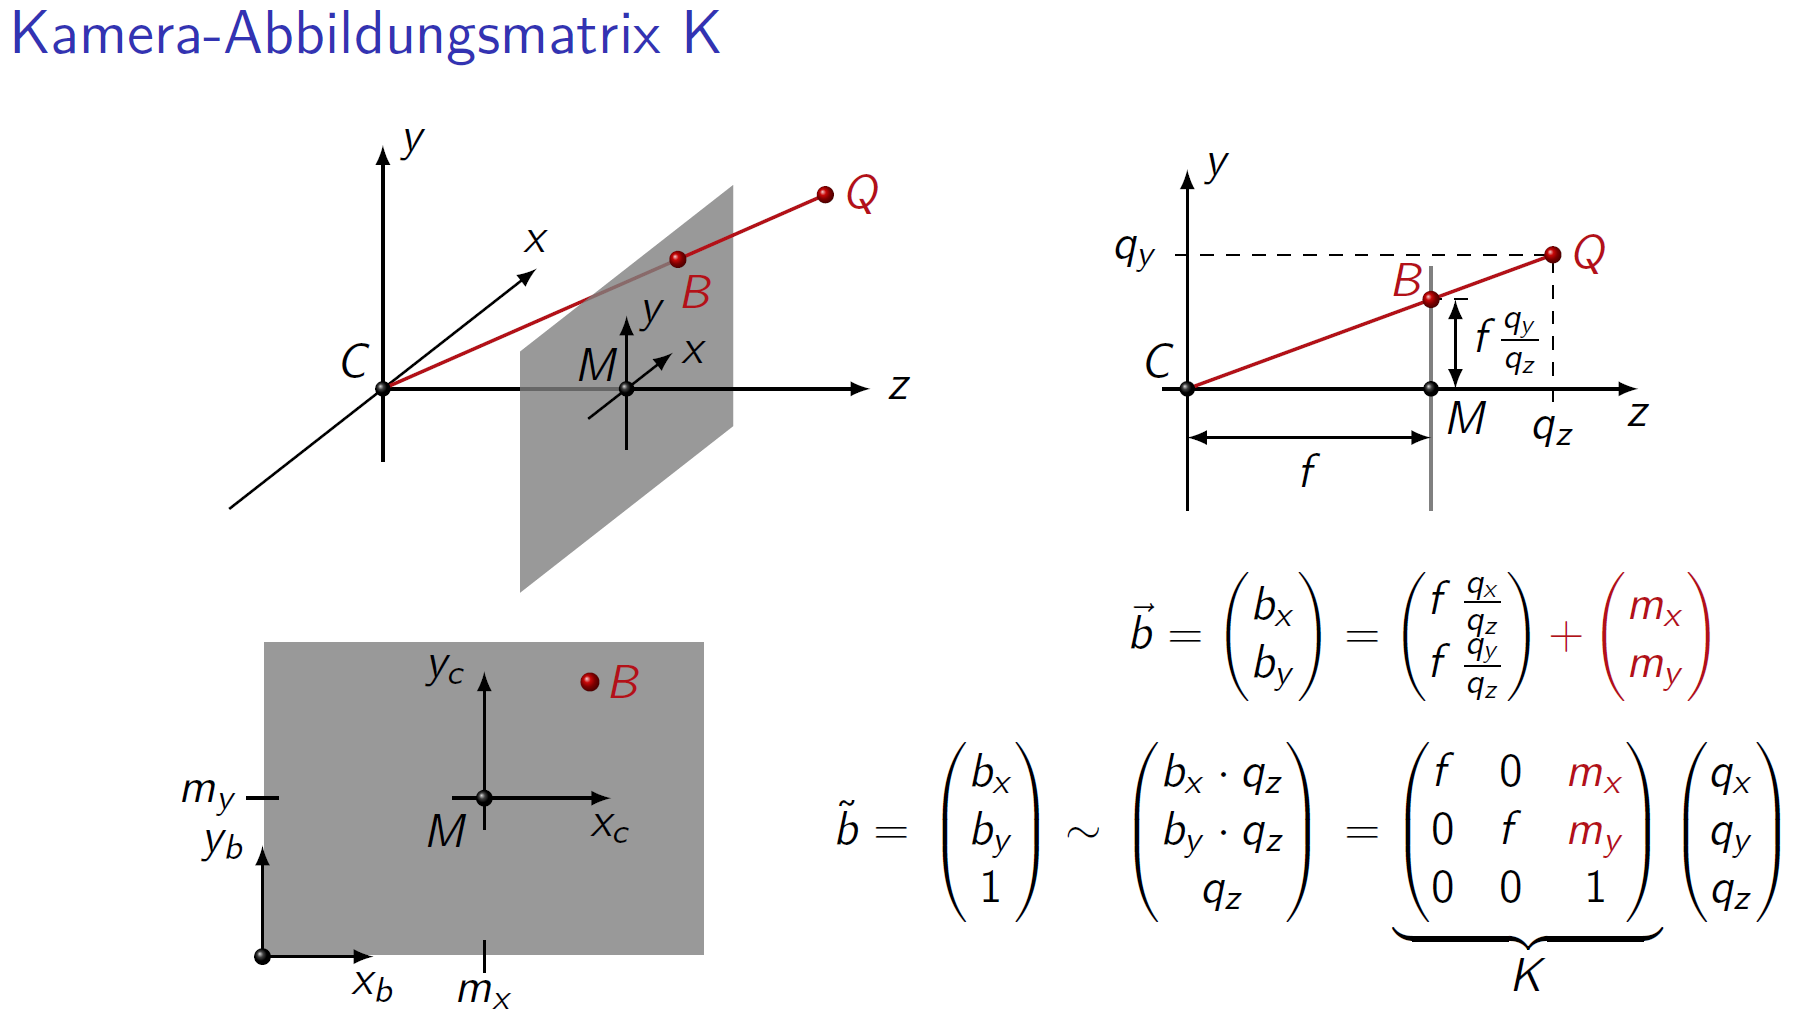
\includegraphics[width=0.8\columnwidth]{images/kamera1.PNG}
	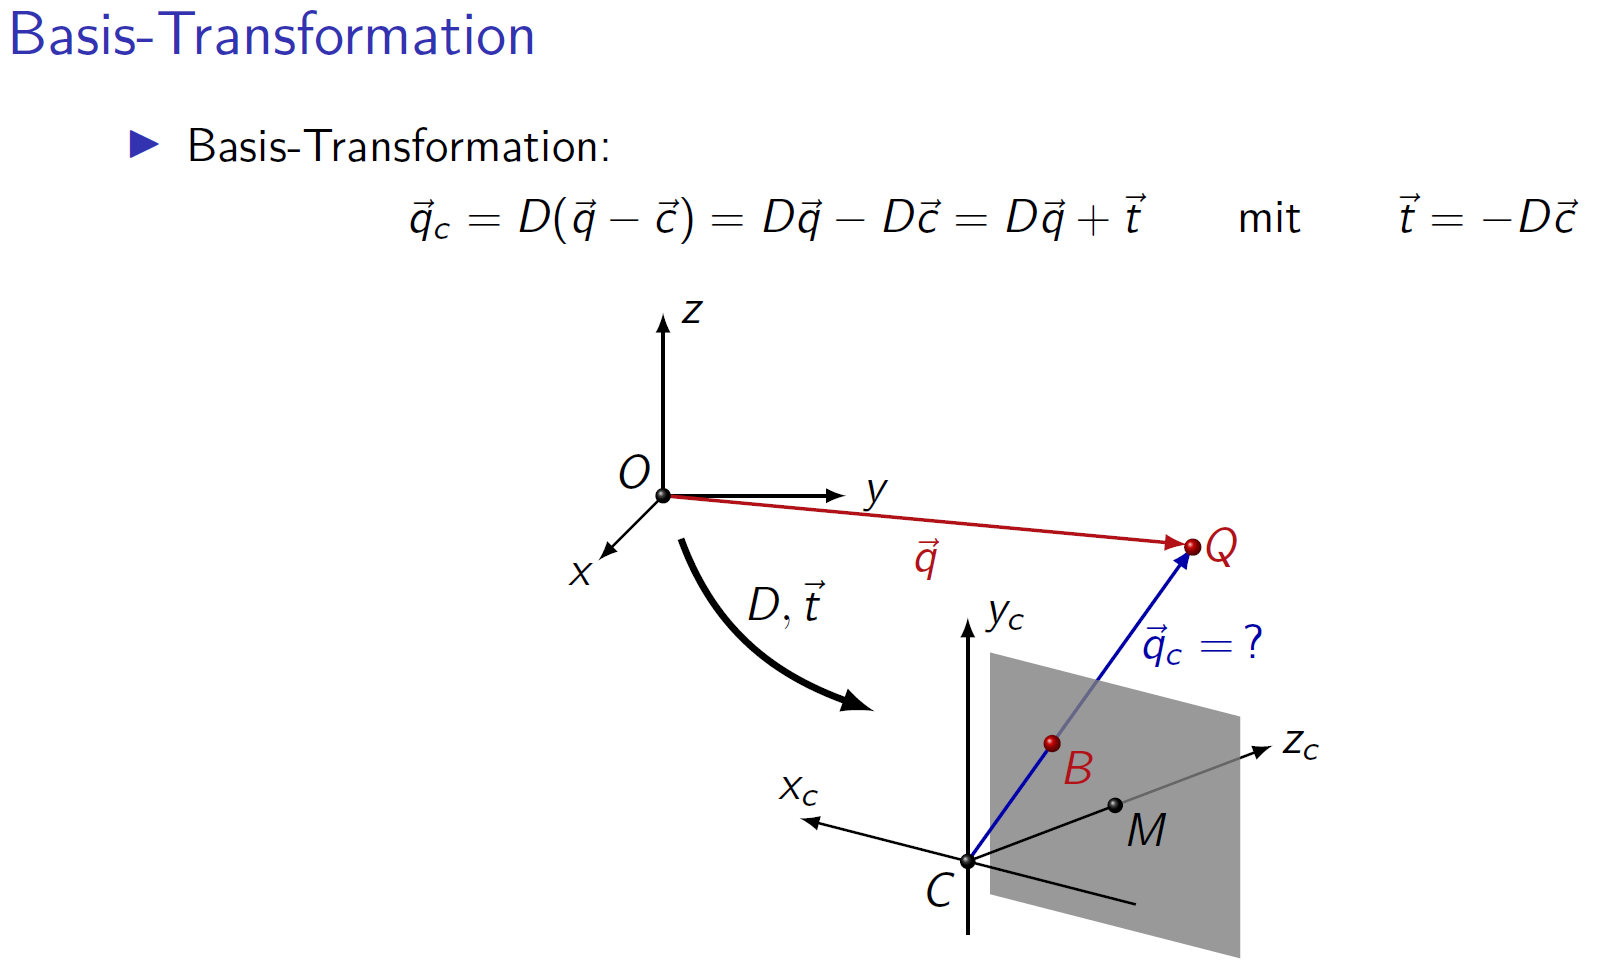
\includegraphics[width=0.8\columnwidth]{images/kamera2.PNG}
	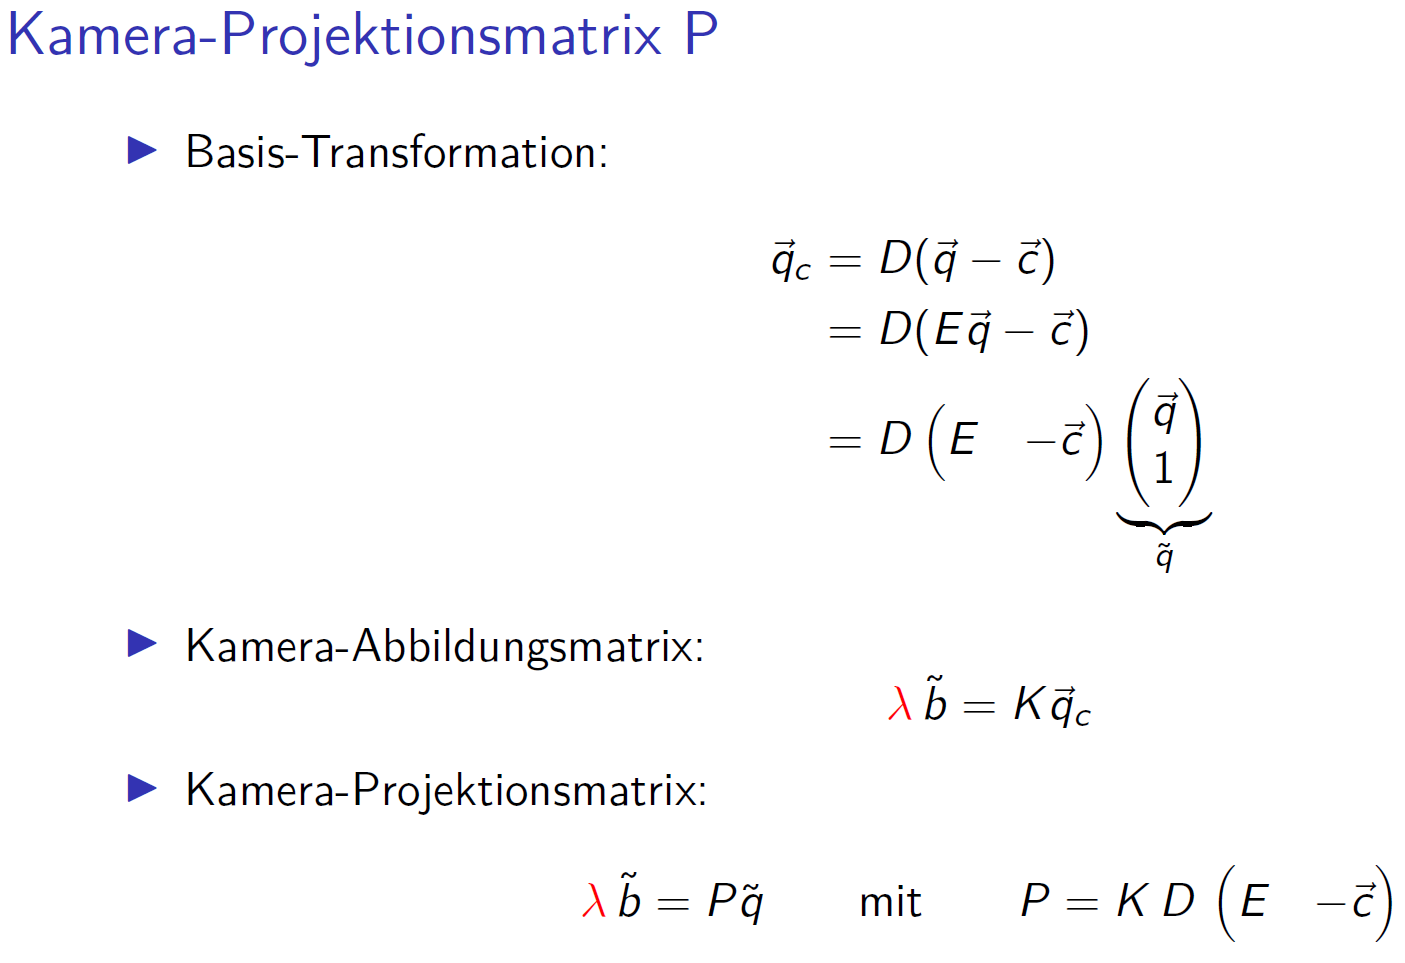
\includegraphics[width=0.8\columnwidth]{images/kamera3.PNG}
	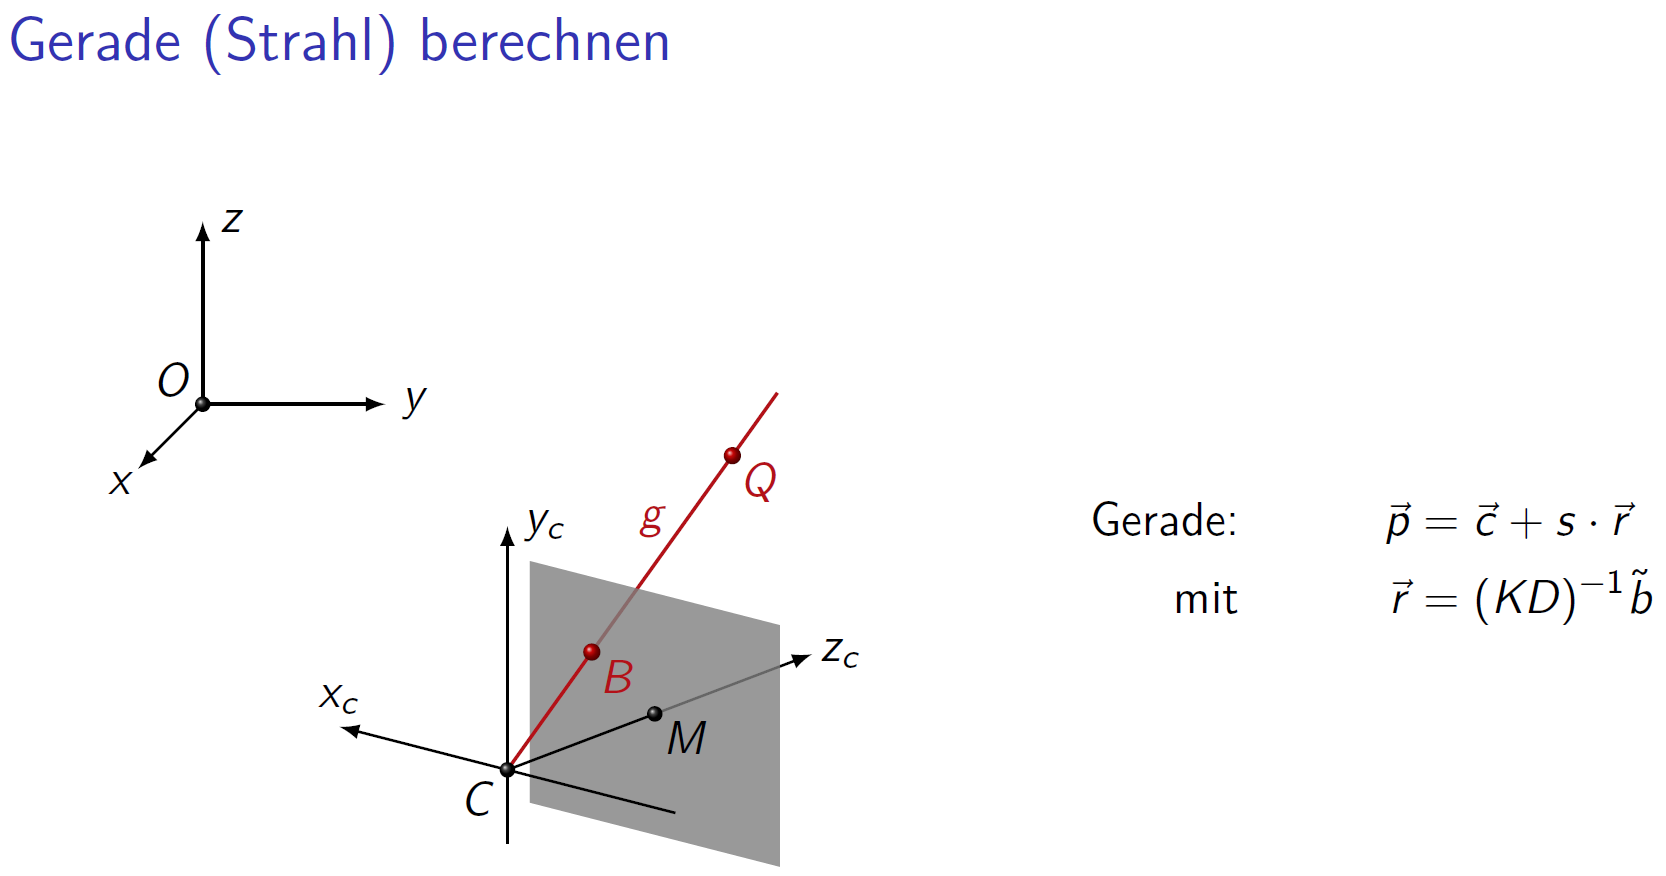
\includegraphics[width=0.8\columnwidth]{images/kamera4.PNG} 
\end{center}
	 

%----------------------------------------------------------------------------------------------
%-------------------------------     7.5 Widerstandsnetzwerk    -------------------------------
%----------------------------------------------------------------------------------------------
\subsection{Widerstandsnetzwerk}

\begin{center}
	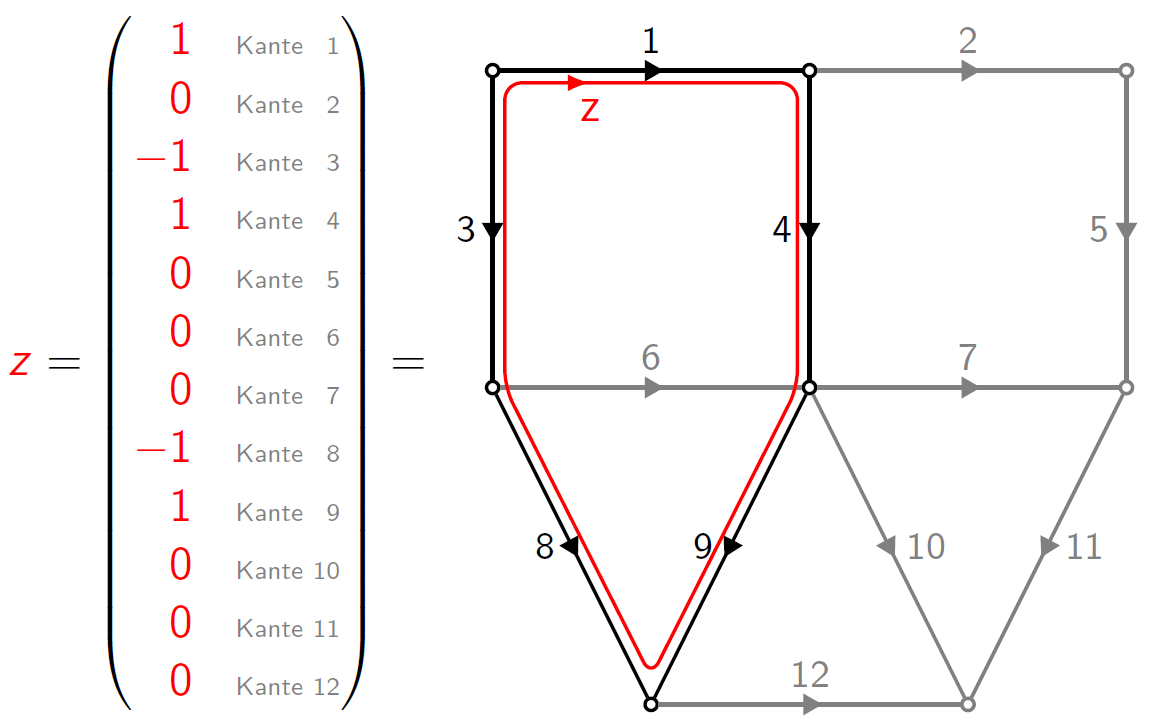
\includegraphics[width=0.8\columnwidth]{images/widerstand1.PNG} 
	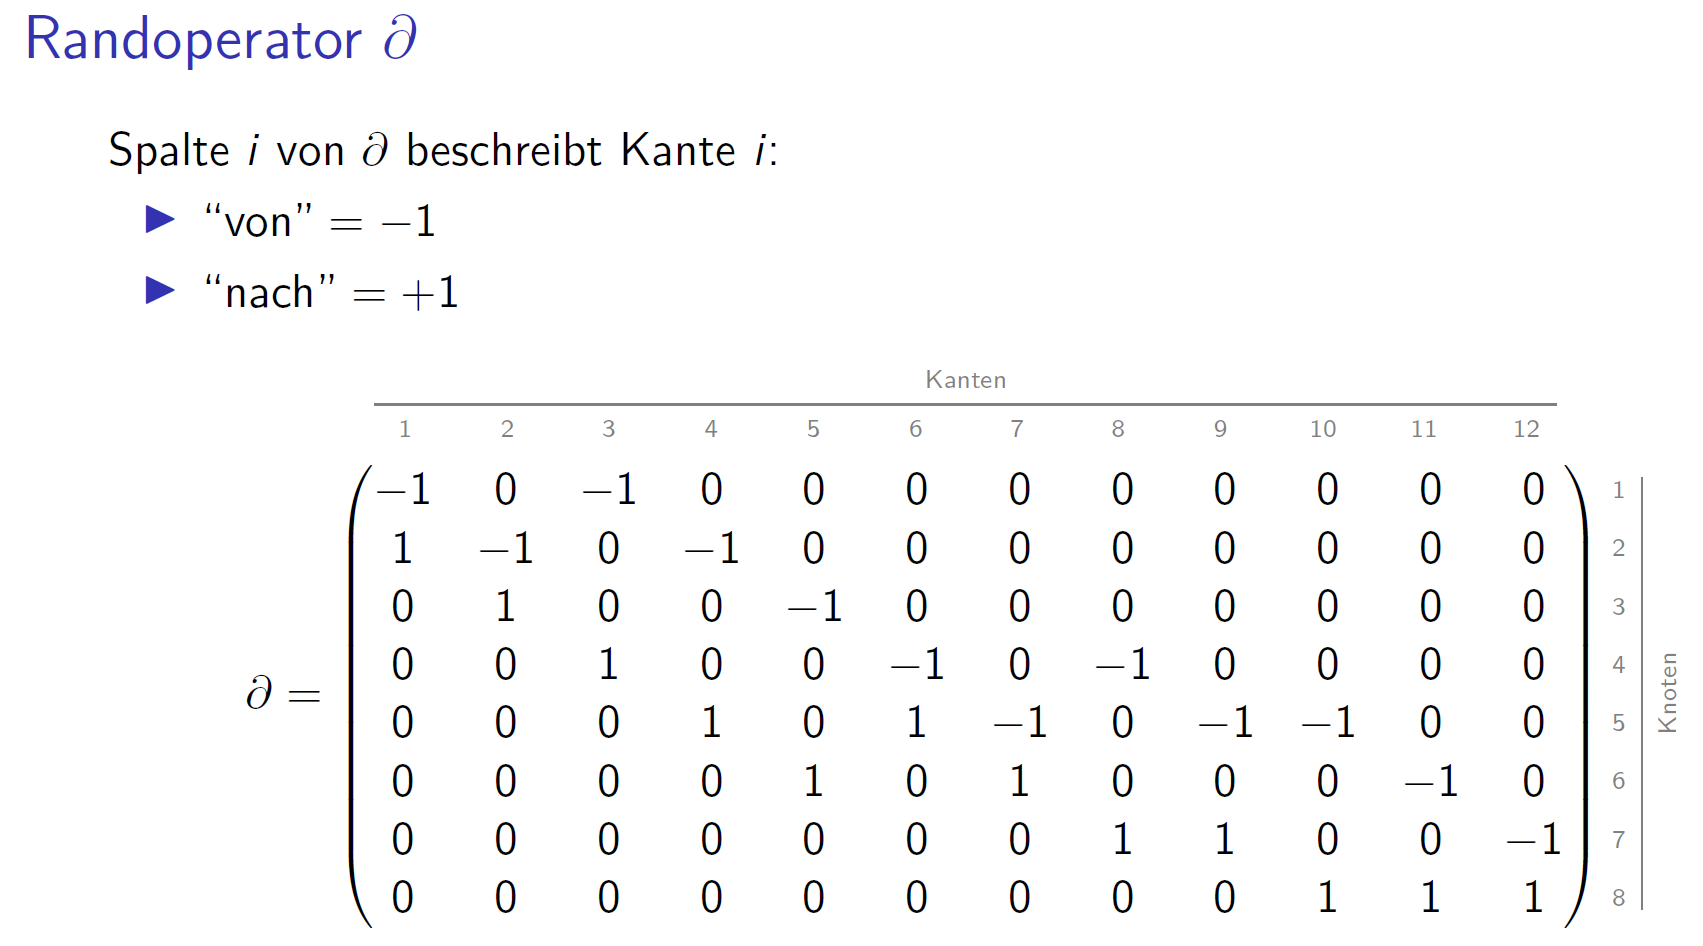
\includegraphics[width=0.8\columnwidth]{images/widerstand2.PNG} 
	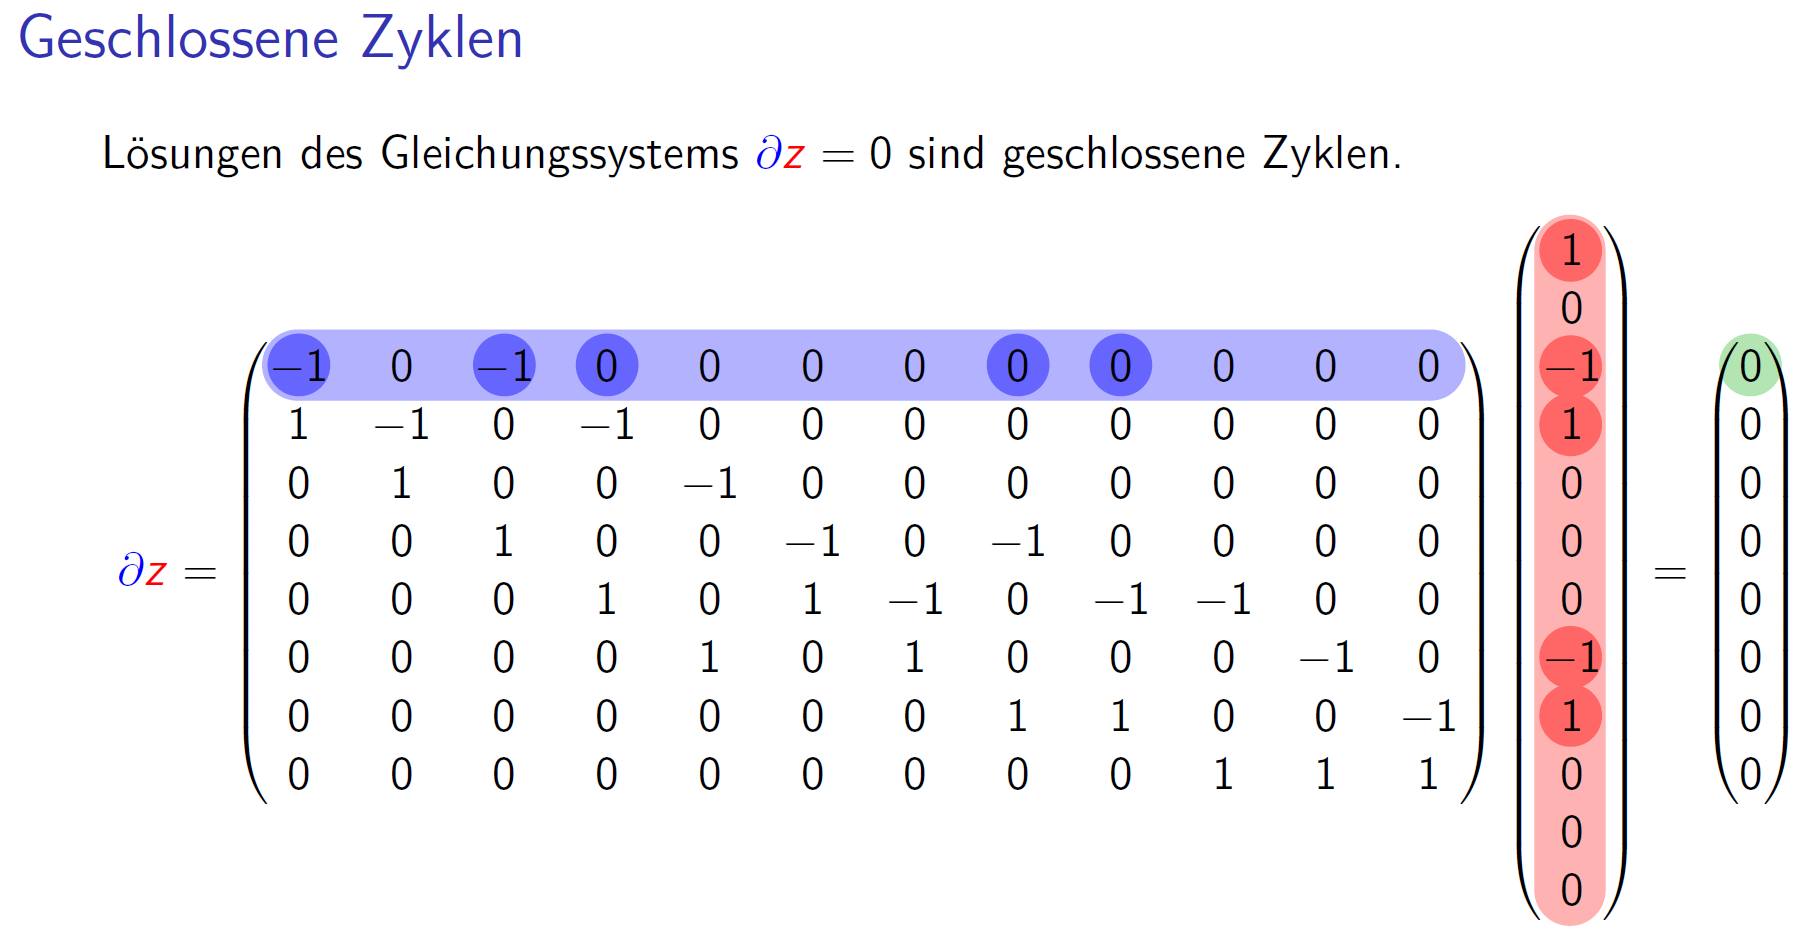
\includegraphics[width=0.8\columnwidth]{images/widerstand3.PNG} 
	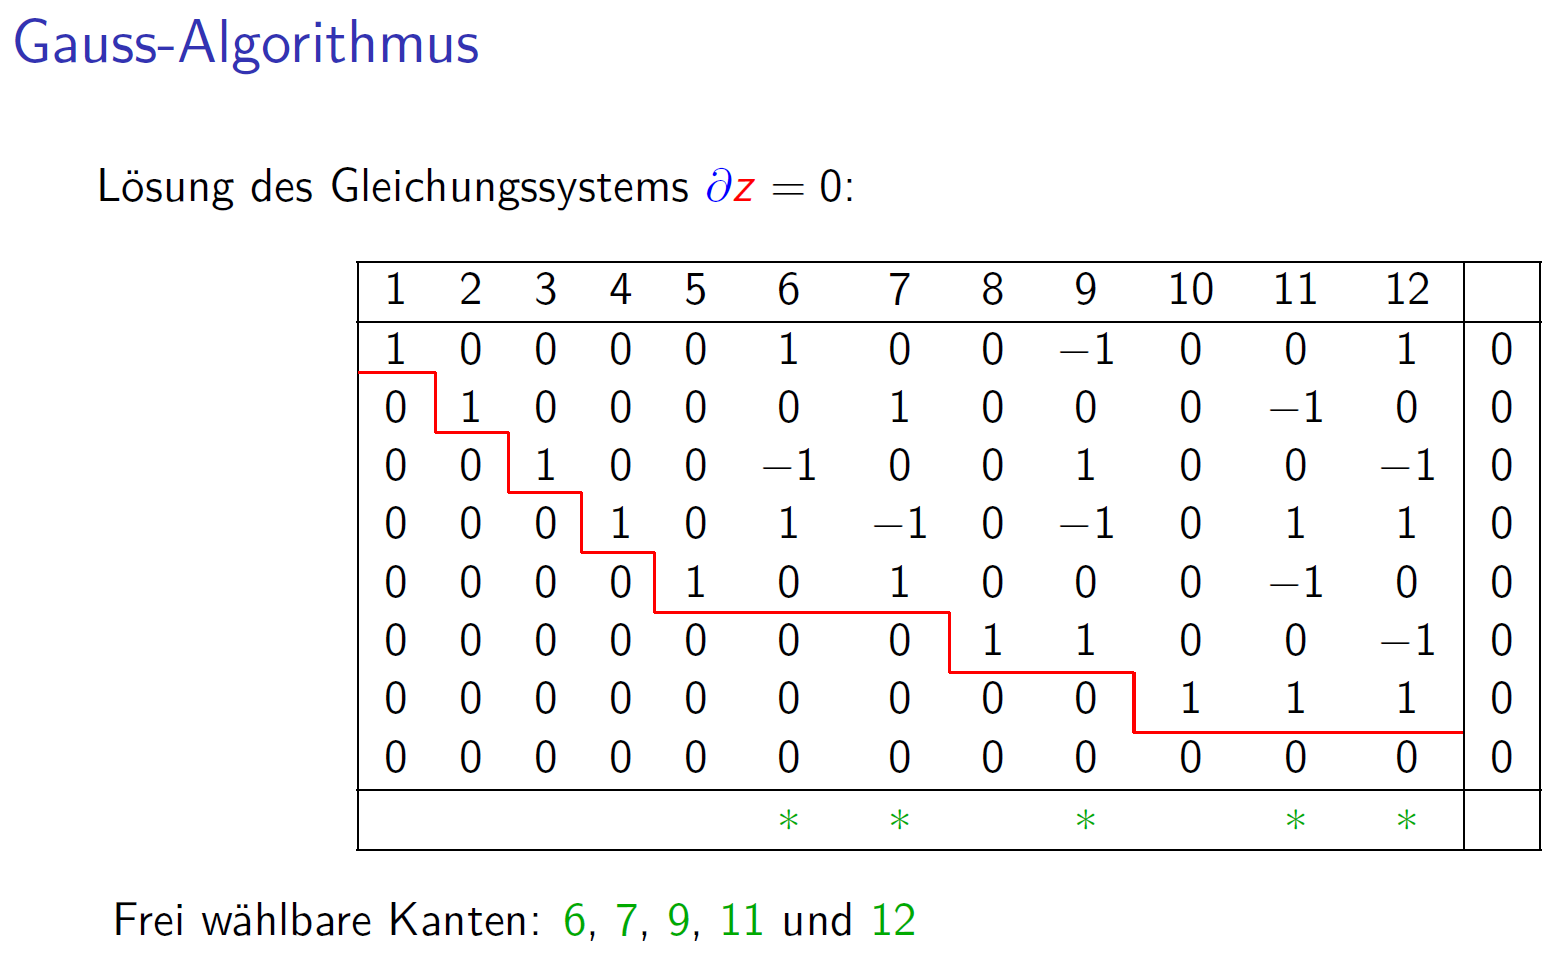
\includegraphics[width=0.8\columnwidth]{images/widerstand4.PNG} 
	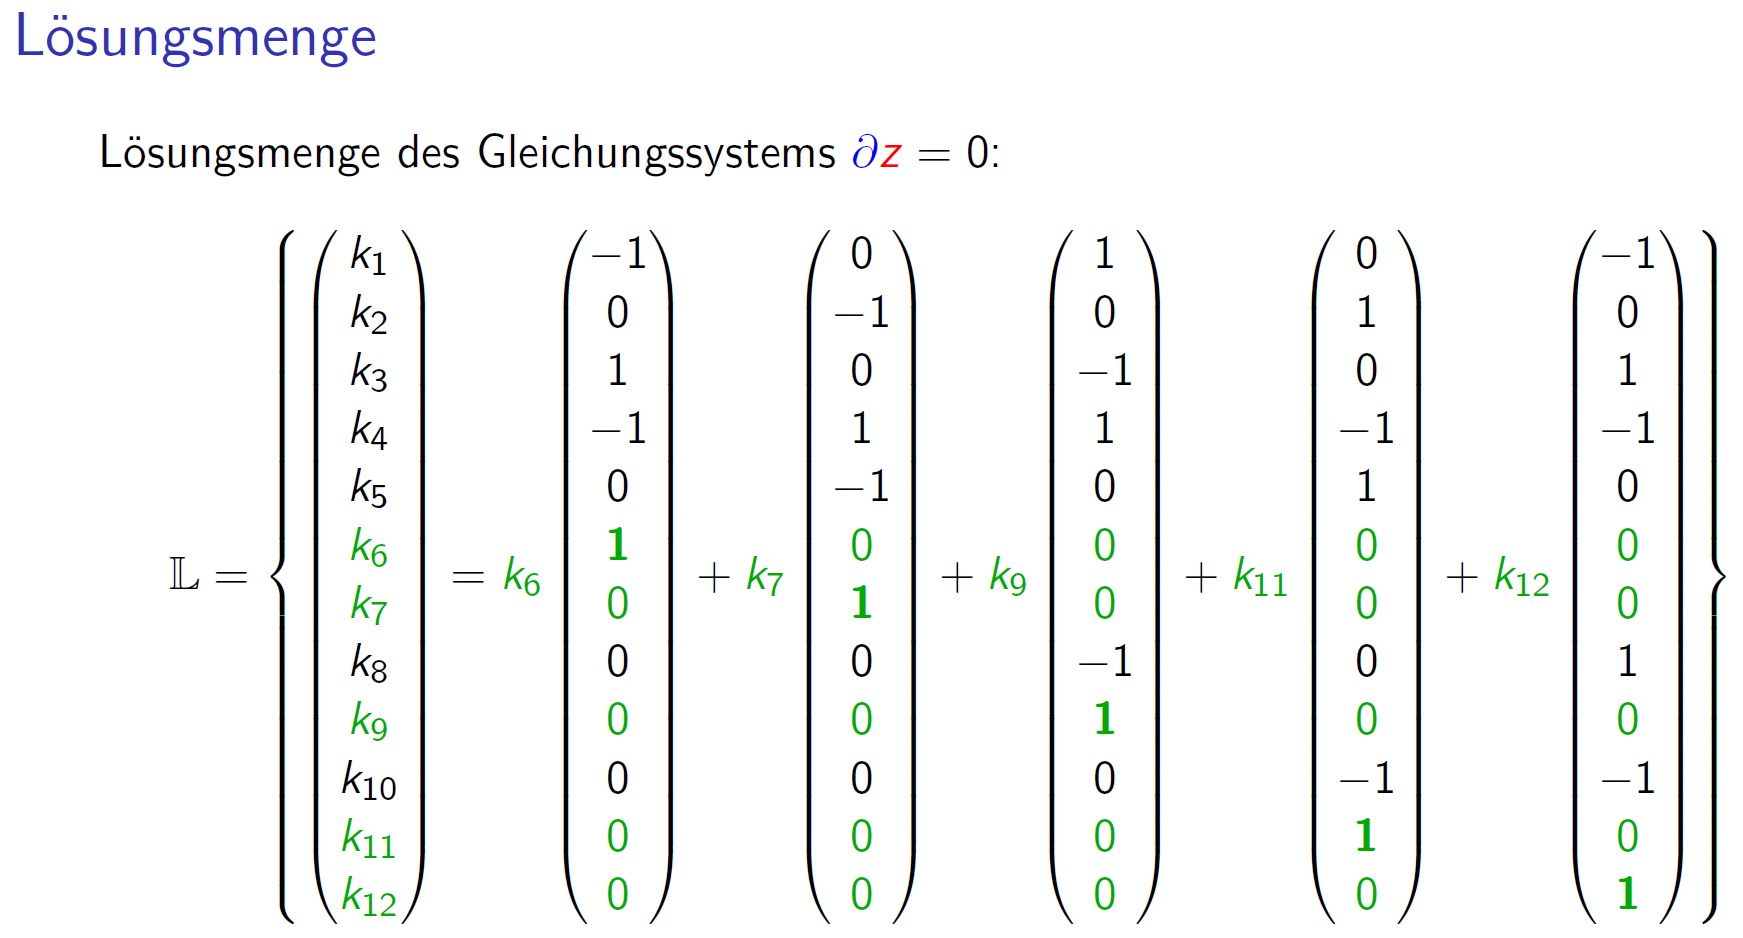
\includegraphics[width=0.8\columnwidth]{images/widerstand5.PNG} 
\end{center}
